%        File: thesis.tex
%     Created: Tue Feb 16 06:00 PM 2016 J
% Last Change: Tue Feb 16 06:00 PM 2016 J
%
%%% jdummy.def
%
\DeclareRelationFont{JY1}{mc}{it}{}{OT1}{cmr}{it}{}
\DeclareRelationFont{JT1}{mc}{it}{}{OT1}{cmr}{it}{}
\DeclareFontShape{JY1}{mc}{m}{it}{<5> <6> <7> <8> <9> <10> sgen*min
    <10.95><12><14.4><17.28><20.74><24.88> min10
    <-> min10}{}
\DeclareFontShape{JT1}{mc}{m}{it}{<5> <6> <7> <8> <9> <10> sgen*tmin
    <10.95><12><14.4><17.28><20.74><24.88> tmin10
    <-> tmin10}{}
\DeclareRelationFont{JY1}{mc}{sl}{}{OT1}{cmr}{sl}{}
\DeclareRelationFont{JT1}{mc}{sl}{}{OT1}{cmr}{sl}{}
\DeclareFontShape{JY1}{mc}{m}{sl}{<5> <6> <7> <8> <9> <10> sgen*min
    <10.95><12><14.4><17.28><20.74><24.88> min10
    <-> min10}{}
\DeclareFontShape{JT1}{mc}{m}{sl}{<5> <6> <7> <8> <9> <10> sgen*tmin
    <10.95><12><14.4><17.28><20.74><24.88> tmin10
    <-> tmin10}{}
\DeclareRelationFont{JY1}{mc}{sc}{}{OT1}{cmr}{sc}{}
\DeclareRelationFont{JT1}{mc}{sc}{}{OT1}{cmr}{sc}{}
\DeclareFontShape{JY1}{mc}{m}{sc}{<5> <6> <7> <8> <9> <10> sgen*min
    <10.95><12><14.4><17.28><20.74><24.88> min10
    <-> min10}{}
\DeclareFontShape{JT1}{mc}{m}{sc}{<5> <6> <7> <8> <9> <10> sgen*tmin
    <10.95><12><14.4><17.28><20.74><24.88> tmin10
    <-> tmin10}{}
\DeclareRelationFont{JY1}{gt}{it}{}{OT1}{cmbx}{it}{}
\DeclareRelationFont{JT1}{gt}{it}{}{OT1}{cmbx}{it}{}
\DeclareFontShape{JY1}{mc}{bx}{it}{<5> <6> <7> <8> <9> <10> sgen*goth
    <10.95><12><14.4><17.28><20.74><24.88> goth10
    <-> goth10}{}
\DeclareFontShape{JT1}{mc}{bx}{it}{<5> <6> <7> <8> <9> <10> sgen*tgoth
    <10.95><12><14.4><17.28><20.74><24.88> tgoth10
    <-> tgoth10}{}
\DeclareRelationFont{JY1}{gt}{sl}{}{OT1}{cmbx}{sl}{}
\DeclareRelationFont{JT1}{gt}{sl}{}{OT1}{cmbx}{sl}{}
\DeclareFontShape{JY1}{mc}{bx}{sl}{<5> <6> <7> <8> <9> <10> sgen*goth
    <10.95><12><14.4><17.28><20.74><24.88> goth10
    <-> goth10}{}
\DeclareFontShape{JT1}{mc}{bx}{sl}{<5> <6> <7> <8> <9> <10> sgen*tgoth
    <10.95><12><14.4><17.28><20.74><24.88> tgoth10
    <-> tgoth10}{}
\DeclareRelationFont{JY1}{gt}{sc}{}{OT1}{cmbx}{sc}{}
\DeclareRelationFont{JT1}{gt}{sc}{}{OT1}{cmbx}{sc}{}
\DeclareFontShape{JY1}{mc}{bx}{sc}{<5> <6> <7> <8> <9> <10> sgen*goth
    <10.95><12><14.4><17.28><20.74><24.88> goth10
    <-> goth10}{}
\DeclareFontShape{JT1}{mc}{bx}{sc}{<5> <6> <7> <8> <9> <10> sgen*tgoth
    <10.95><12><14.4><17.28><20.74><24.88> tgoth10
    <-> tgoth10}{}
\DeclareRelationFont{JY1}{gt}{it}{}{OT1}{cmr}{it}{}
\DeclareRelationFont{JT1}{gt}{it}{}{OT1}{cmr}{it}{}
\DeclareFontShape{JY1}{gt}{m}{it}{<5> <6> <7> <8> <9> <10> sgen*goth
    <10.95><12><14.4><17.28><20.74><24.88> goth10
    <-> goth10}{}
\DeclareFontShape{JT1}{gt}{m}{it}{<5> <6> <7> <8> <9> <10> sgen*tgoth
    <10.95><12><14.4><17.28><20.74><24.88> tgoth10
    <-> tgoth10}{}
\endinput
%%%% end of jdummy.def

%\documentclass[submit]{ipsj_v2/UTF8/ipsj}
%\documentclass{ipsj}
%\documentclass[submit,techrep]{ipsj_v2/UTF8/ipsj}
\documentclass[submit,techrep]{ipsj}

\usepackage{color}
\usepackage{latexsym}
\usepackage[dvipdfmx]{graphicx}
\usepackage{amssymb}
\usepackage{enumerate,cite,url}
\usepackage{listings,jlisting}
\lstset{%
    language={c},%
    basicstyle={\small},%
    identifierstyle={\small},%
    commentstyle={\scriptsize\itshape},%
    keywordstyle={\small},%\bfseries},%
    ndkeywordstyle={\small},%
    stringstyle={\small\it},
    frame={tb},
    breaklines=true,
    columns=[l]{fullflexible},%
    numbers=left,%
    xrightmargin=0zw,%
    xleftmargin=3zw,%
    numberstyle={\scriptsize},%
    stepnumber=1,
    numbersep=1zw,%
    lineskip=-1.5ex%
}

\def\Underline{\setbox0\hbox\bgroup\let\\\endUnderline}
\def\endUnderline{\vphantom{y}\egroup\smash{\underline{\box0}}\\}
\def\|{\verb|}

\setcounter{巻数}{53}%vol53=2012
\setcounter{号数}{10}
\setcounter{page}{1}

\begin{document}

\title{Bluetoothを用いたマルチVM対応\\mrubyバイトコードローダ}

\etitle{mruby Bytecode Loader Using Bluetooth in Multi-VM Environment}

\affiliate{OU}{大阪大学基礎工学部\\
School of Engineering Science, Osaka University}

\affiliate{OKUMA}{オークマ株式会社\\
OKUMA Corporation}

\affiliate{GOU}{大阪大学基礎工学研究科\\
Graduate School of Engineering Science, Osaka University}

\author{山本 拓朗}{Takuro Yamamoto}{OU}%[joho.taro@ipsj.or.jp]
\author{大山 博司}{Hiroshi Oyama}{OKUMA}%
\author{安積 卓也}{Takuya Azumi}{GOU}%[gakkai.jiro@ipsj.or.jp]

\begin{abstract}
近年,組込みシステムは複雑化・大規模化しているため,ソフトウェアの生産性が問題になっている.
組込みソフトウェア開発の生産性の向上を目的として,mruby(軽量Ruby)を適用させたコンポーネントベース開発が可能なフレームワークであるmruby on TECSを提案してきた.
現状のmruby on TECSでは,プラットフォームにmrubyバイトコードを組み込んでいるため,mrubyプログラムを修正する度にコンパイル・リンクし直す必要がある.
さらに,マルチVMを提供しているが,複数のmrubyプログラムを効率よく並行動作させるには開発者がリアルタイムOSの機能を熟知している必要がある.
本研究では,mruby on TECSの拡張として,mrubyアプリケーションのバイトコードをBluetoothで転送することで開発効率を向上させる.
さらに,複数のmrubyプログラムを協調動作できるフレームワークを提案する.

\end{abstract}

% \begin{jkeyword}
% 情報処理学会論文誌ジャーナル,\LaTeX,スタイルファイル,べからず集
% \end{jkeyword}

\begin{eabstract}
In recent years, the productivity of embedded systems has become a problem due to their complexity and large-scale.
For the purpose of improving the productivity for embedded software development, the mruby on TECS framework has been proposed that is applied mruby (Lightweight Ruby) and supports component-based development.
In the current mruby on TECS, the mruby programs have to be compiled and linked every time the programs are modified because the mruby bytecodes are incorporated in the platform.
Moreover, while the framework supports multi-VM, developers need to be familiar with the functions of RTOSs to effectively execute multiple mruby programs in concurrent or/and parallel.
To improve the development efficiency, this paper proposes an mruby bytecode loader using Bluetooth as an extension of mruby on TECS.
In addition, multiple mruby programs cooperatively run in the proposed framework.
A RiteVM sceduler makes multitasking processing more easy-to-use than that of mruby on TECS.
\end{eabstract}

% \begin{ekeyword}
% IPSJ Journal, \LaTeX, style files, ``Dos and Don'ts'' list
% \end{ekeyword}

\maketitle

\section{はじめに}
\vspace{-2mm}
近年,組込みシステムは高品質・高性能化に伴い,複雑化・大規模化している上に,製品の低コスト化や短期間での開発も要求されている.

ソフトウェアを効率的に開発するアプローチに,コンポーネントベース開発がある.
%コンポーネントベース開発は,再利用可能なコンポーネントを構成するための設計手法である.
コンポーネント化されたソフトウェアは,再利用性が高く,検証が容易になるため,複雑・大規模なソフトウェアを効率的に開発できる.
システムの拡張や仕様変更に柔軟に対応できる.
組込みシステムのコンポーネント技術として,TECS (TOPPERS Embedded Component System)\cite{par:TECS}やAUTOSAR\cite{url:AUTOSAR}がある.

効率的なソフトウェア開発のもう一つのアプローチとして,スクリプト言語がある.
現在の組込みソフトウェアのほとんどはC言語で開発されているが,C言語による開発はコストが高く,開発期間も長くなる.
スクリプト言語は,その使いやすさから高い生産性を持っているため,効率的かつ短期間での開発ができる.
有名なスクリプト言語として,Ruby, Perl,Python,Luaなどがある.

しかし,スクリプト言語は生産性が高い反面,C言語よりも実行時間が遅い.
組込みシステムにとって,デッドラインを守るといったリアルタイム性は重要であるため,スクリプト言語を組込みシステムに利用することは難しい.

%mruby on TECSは,スクリプト言語であるmruby使用したコンポーネントベース開発が可能なフレームワークである\cite{par:mrubyonTECS}.
mruby on TECS は,mruby(軽量Ruby)\cite{par:mruby}と,組込みシステムに適したコンポーネントシステムであるTECSを組み合わせたフレームワークである\cite{par:mrubyonTECS}.
mruby on TECS では,mruby プログラムからC 言語の関数を呼ぶ機能を提供しており,mruby に比べて,アプリケーションを約100 倍速く実行できる.

現状のmruby on TECSでは,いくつかの問題がある.
mruby on TECS は,mrubyプログラムをロードするための方法として,SDカードやROMへの書き込みにしか対応していないため,作業効率が悪い.
例えば,LEGO MINDSTORMS EV3 のプラットフォーム\cite{par:EV3}を利用した場合,mrubyプログラムを修正する度に,SDカードの抜き差しを行う必要がある.
%mruby on TECS では,mruby プログラムを修正する度にターゲットデバイスでSD カードまたはROMに書き込みし,OS を再起動する必要がある.
さらに,mruby on TECS はマルチVMに対応してるが,複数のmruby アプリケーションを並行実行させる場合,開発者がタスクを待ち状態へ遷移させるOS の機能を呼び出さなければならない.

% mrubyバイトコードローダによって,開発者ははじめの一度だけ記憶装置にプラットフォーム部分を書き込み,mrubyアプリケーションのバイトコードをホストからターゲットデバイスへBluetoothを用いて転送し,実行することが可能になる.
% 繰り返してSDカードの抜き差しやROMへの書き込みをする手間が省けるため,作業効率は向上する.
% RiteVMスケジューラは複数のmrubyアプリケーションを
本論文では,上記の問題を解決するため,mruby on TECSを拡張して,Bluetoothを用いたmrubyバイトコードローダおよびRiteVMスケジューラを提案する.
% 提案フレームワークでは,プラットフォーム部分をコンパイル・リンクし,ターゲットデバイス上で起動する.
% ホストPC 側では,mruby アプリケーション(.rb) をバイトコード(.mrb) にコンパイルし,Bluetooth を通してターゲットデバイスにバイトコードを転送する. 
% ターゲットデバイス側では,RiteVM に実装されたローダが転送されたバイトコードを受信し,すでにプラットフォームに含まれているmruby ライブラリと合わせてアプリケーションを実行する.
% これによって,繰り返しSDカードの抜き差しやROMへの書き込みをする手間やOSを再起動する時間が省けるため,作業効率を上げることができる.
% RiteVMに実装されたローダが,ホストから転送されたバイトコードを受信し,アプリケーションを実行する.
% これによって,繰り返しSDカードの抜き差しやROMへの書き込みをする手間やOSを再起動する時間が省けるため,作業効率を上げることができる.
% さらに,各VM の処理を平等に実行するRiteVM スケジューラを提供することで,マルチタスク処理を効率的に利用できる.

本論文における貢献は次のとおりである.
mrubyバイトコードローダの実装により,mruby on TECSを使ったソフトウェア開発における作業効率を向上させる.
RiteVMスケジューラの実装により,複数のmrubyプログラムを効率的に並行・並列動作させる.
コンポーネントベース開発の利点を明らかにする.
% Contribution: The proposed framework gives the contribution in the following points.
% 1) To improve the software development efficiency:
% Developers do not need to rewrite a storage/ROM device and also to restart an OS. 
% The loader supports the countinuous loading, which saves the Bluetooth setup time. 
% Therefore, the mruby bytecode loader using Bluetooth helps developers develop software.
% 2) To effectively execute multiple mruby programs in concurrent or/and parallel: 
% Developers can execute multiple tasks without the knowledge of an RTOS because the RiteVM sceduler switches tasks cyclically.
% In additon, synchronization of multiple tasks is also implemented.
% 3) To focus on the benefits of component-based developments:
% This paper shows the specific examples for the benefits of component-based development.

本論文の構成を次に述べる.
まず\ref{sec:Background}章で,提案フレームワークのベースであるmruby on TECSについて述べる.
\ref{sec:Design and Implementation}章では,提案フレームワークの設計と実装について述べる.
\ref{sec:Evaluation}章では,提案フレームワークの作業効率や実行時間のオーバヘッドを評価する.
\ref{sec:Related Work}章では,関連研究について述べる.
最後に,\ref{sec:Conclusion}章で本論文をまとめる.

% Organization: The paper is organized as follows. 
% Section 2 introduces the basic technologies i.e. mruby, TECS and mruby on TECS. 
% Section 3 describes the design and implementation of the proposed framework in detail. 
% Section 4 evaluates the proposed framework, Section 5 discusses related work, and then Section 6 concludes this paper.

 \section{mruby on TECS (既存フレームワーク)}
\vspace{-2mm}
\label{sec:Background}
% 図\ref{fig:proposed}に提案フレームワークのシステムモデルを示す.
% RiteVMとmrubyライブラリを含むプラットフォーム部分は,はじめにターゲットデバイス上で起動されている.
% mrubyアプリケーションのバイトコードは,ホストからターゲットデバイスへと転送される.
% それぞれバイトコードは,RiteVMに割り当てられ,並行して起動される.
%
この章では,提案フレームワークのベースになっているmruby on TECSについて述べる.
mruby on TECSで利用されているmrubyとTECSについても述べる.
% \begin{figure}[t]
%     \centering
%     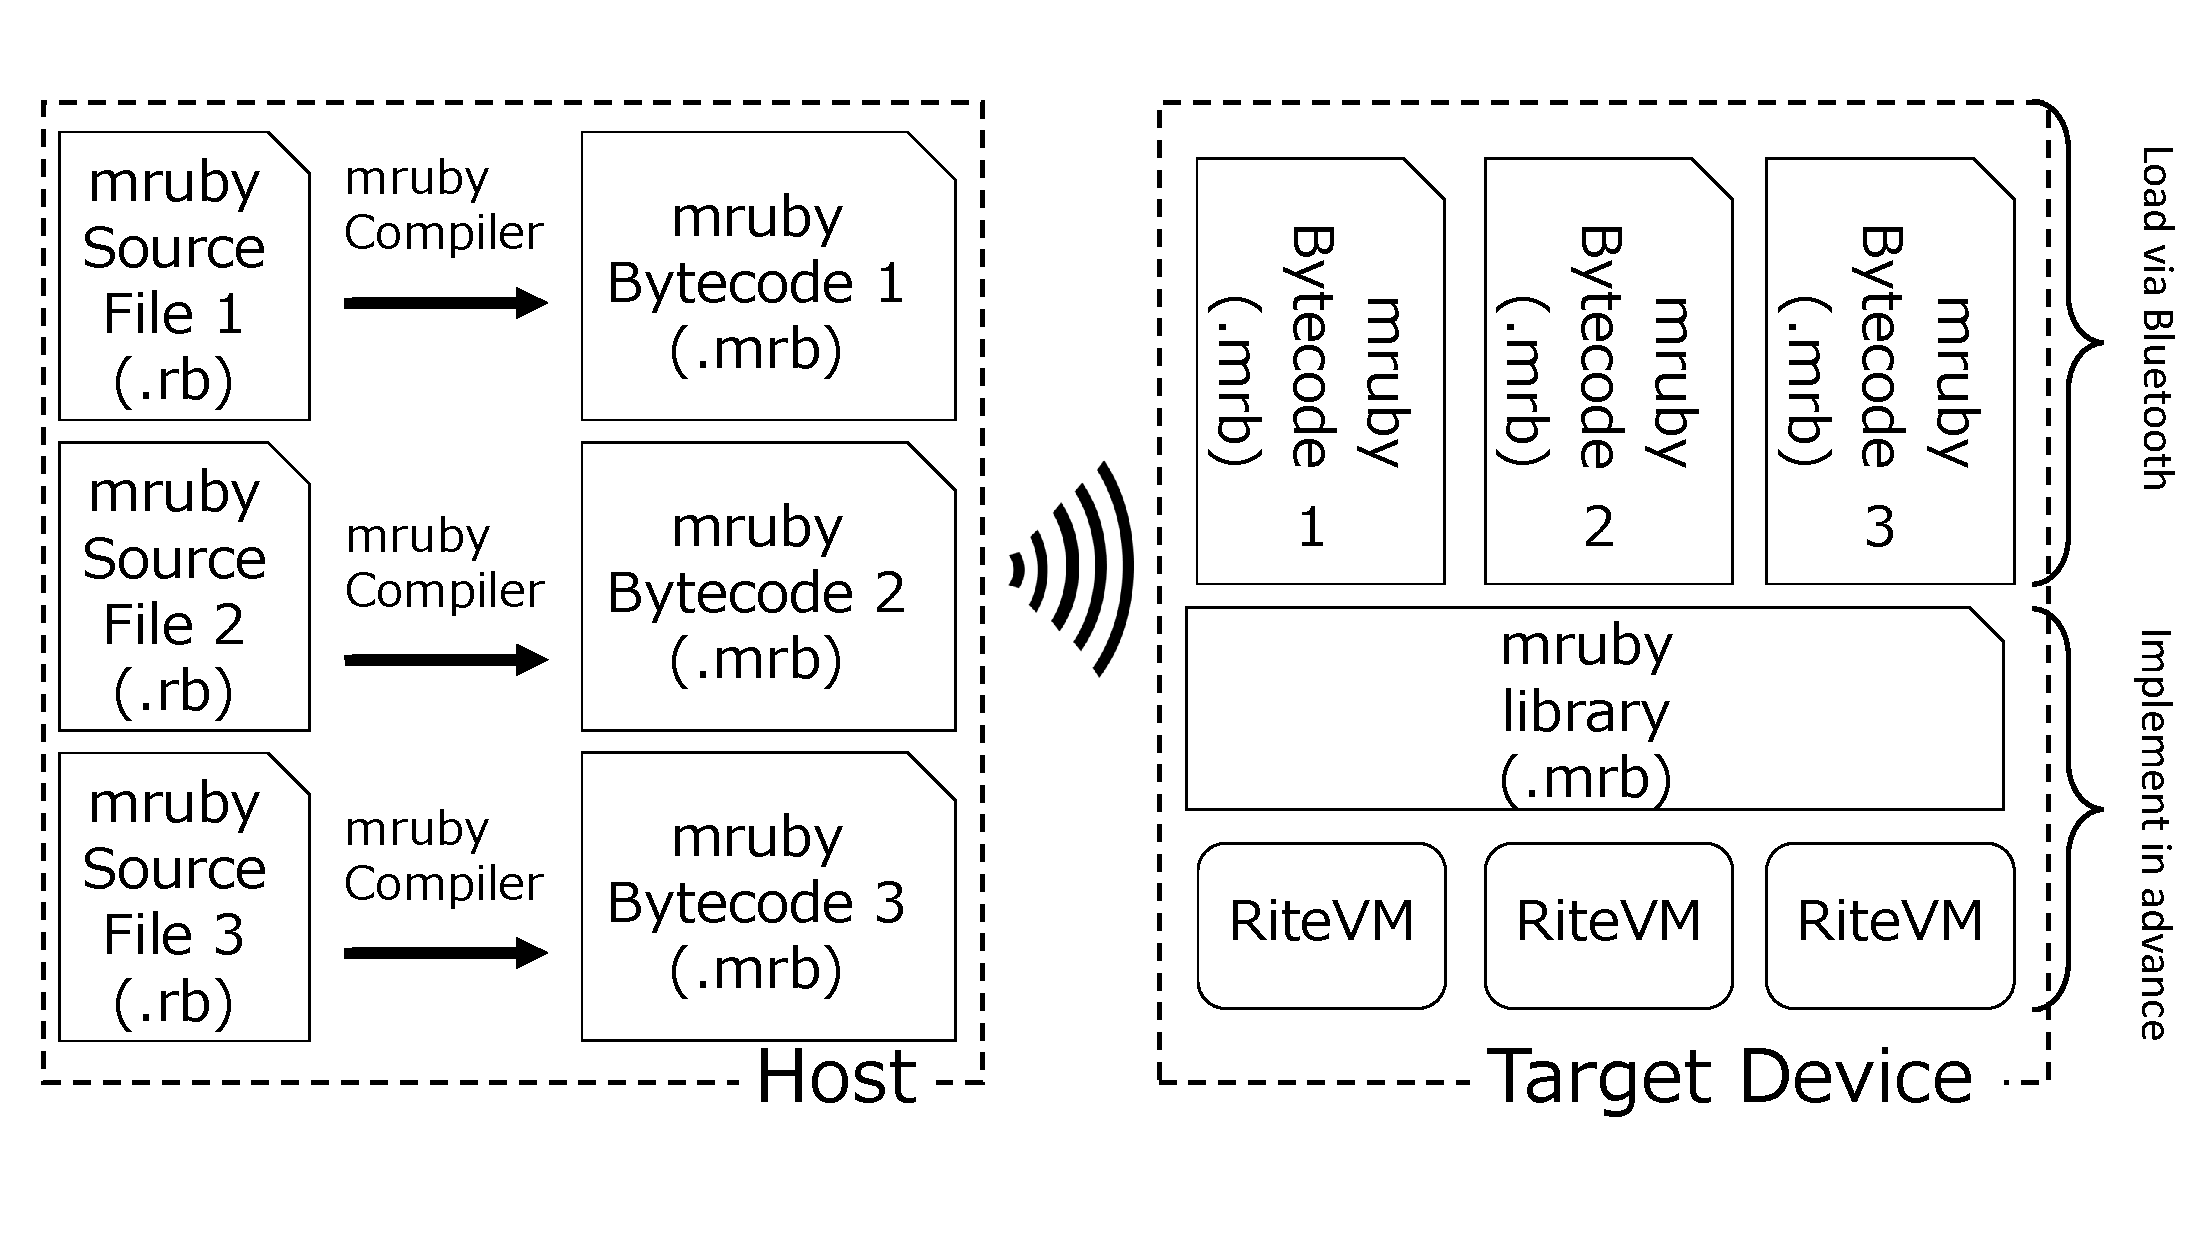
\includegraphics[width=8cm,clip]{../EMSOFT2016/figure/proposed.pdf}
%     \caption{システムモデル}
%     \label{fig:proposed}
% \end{figure}

\subsection{mruby}
% mrubyは,ISO規格の一部に準拠したRubyの軽量実装である.
% Ruby\cite{url:Ruby}は,オブジェクト指向型のスクリプト言語である.
% 特徴としてシンプルな文法なため読みやすくかつ使いやすい上に,C言語よりも少ないコード量で記述できる.
% 他にも,クラスやメソッドといったオブジェクト指向関数,例外,ガベージコレクションなどの機能により,生産性を向上させることができる.

mrubyは,Rubyの可読性や使いやすさはそのままに,リソースが少なく起動が速いため,組込みシステムに適している.
mrubyには,RiteVMと呼ばれるVMが実装されているため,どのOS上でもアプリケーションを起動させることができる.
%図\ref{fig:mruby}にRiteVMのメカニズムを示す.
mrubyコンパイラは,mrubyプログラム(.rb)を,中間言語であるバイトコード(.mrb)にコンパイルする.
RiteVMが実装されていれば,どのターゲットデバイス上でも同じmrubyプログラムを実行できる.

% \begin{figure}[t]
%     \centering
%     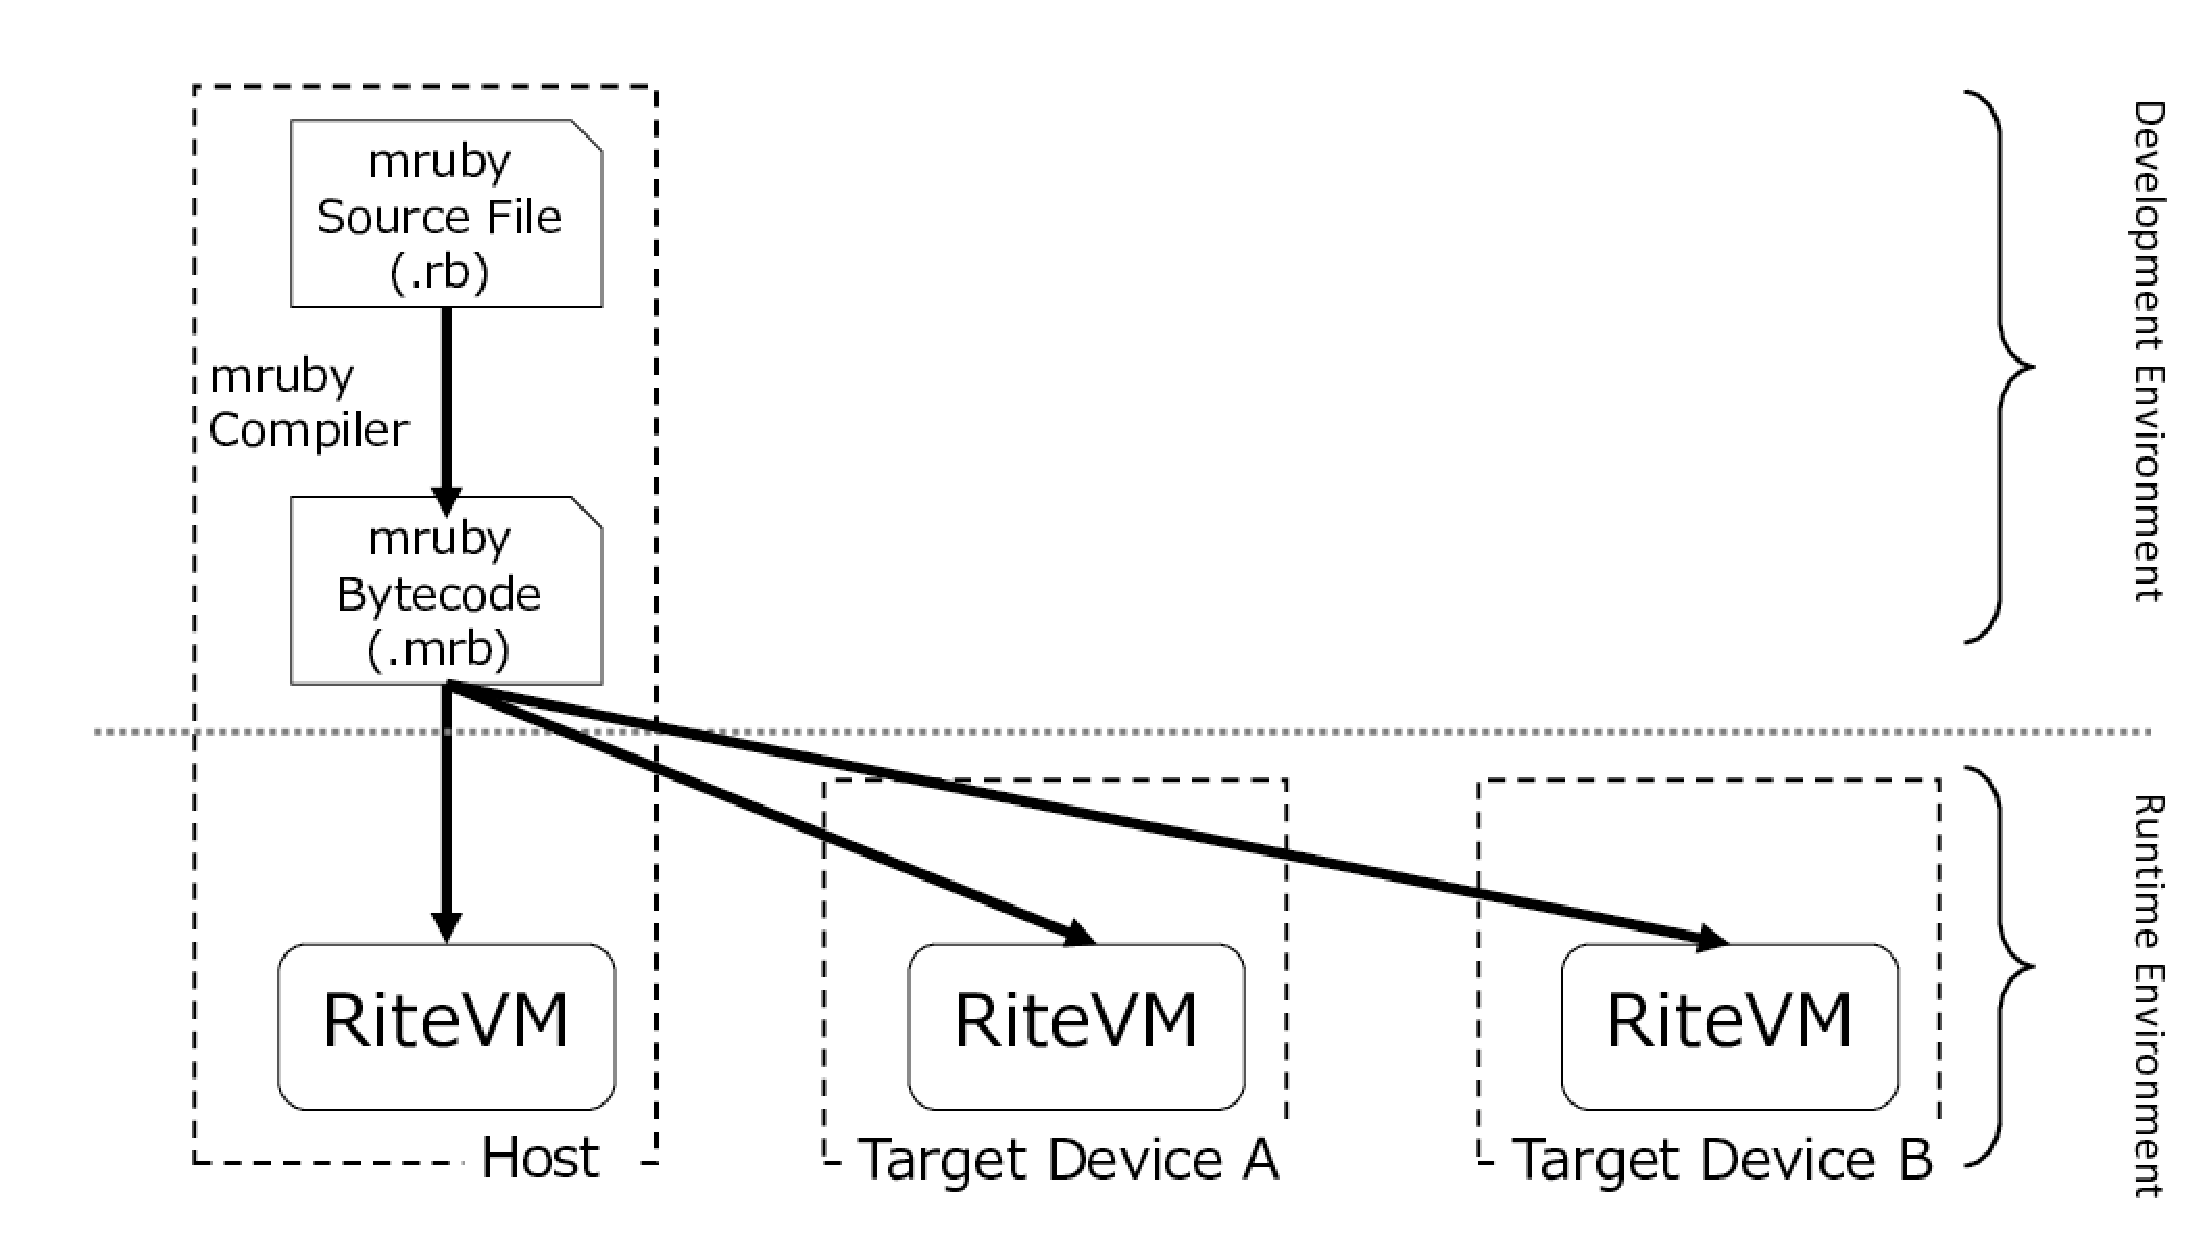
\includegraphics[width=8cm,clip]{../EMSOFT2016/figure/mruby.pdf}
%     \caption{Mechanism of mruby/RiteVM}
%     \label{fig:mruby}
% \end{figure}

\subsection{TECS\cite{par:TECS}}
%TECSは,組込みシステム向けのコンポーネントシステムである.
TECSによるコンポーネントベース開発は,ソフトウェアの再利用性を上げるため,生産性を向上できる.
%システム全体の構造を可視化するため,システムの難しさを減らすことができる.
%ソフトウェアの共通部分はコンポーネントとして扱われるため,開発の重複を減らし,生産性を向上させる.

% TECSでのコンポーネントの生成と結合は静的に行われるため,最適化され,実行時間や消費メモリのオーバヘッドは少ない.
% 他の特徴として,C言語での実装,ソースレベルでの移植性,コンポーネントの粒度が小さいことなどがある.

\subsubsection{コンポーネントモデル}
図\ref{fig:component}にコンポーネント図の例を示す.
TECSでは,インスタンス化されたコンポーネントはセル({\it cell})と呼ばれ,受け口({\it entry}),呼び口({\it call}),属性,変数を持つ.
受け口は自身の機能を提供するインタフェースで,呼び口は他のセルの機能を利用するためのインタフェースである.
セルは複数の受け口や呼び口を持つことができる.
セルの提供する関数は,C言語で実装される.

受け口と呼び口の型は,セルの機能を使うためのインタフェースであるシグニチャによって定義される.
セルの呼び口は,同じシグニチャを持つ他のセルの受け口と結合できる.
セルの型は,セルタイプと呼ばれ,受け口,呼び口,属性,変数の組を定義している.

\begin{figure}[t]
    \centering
    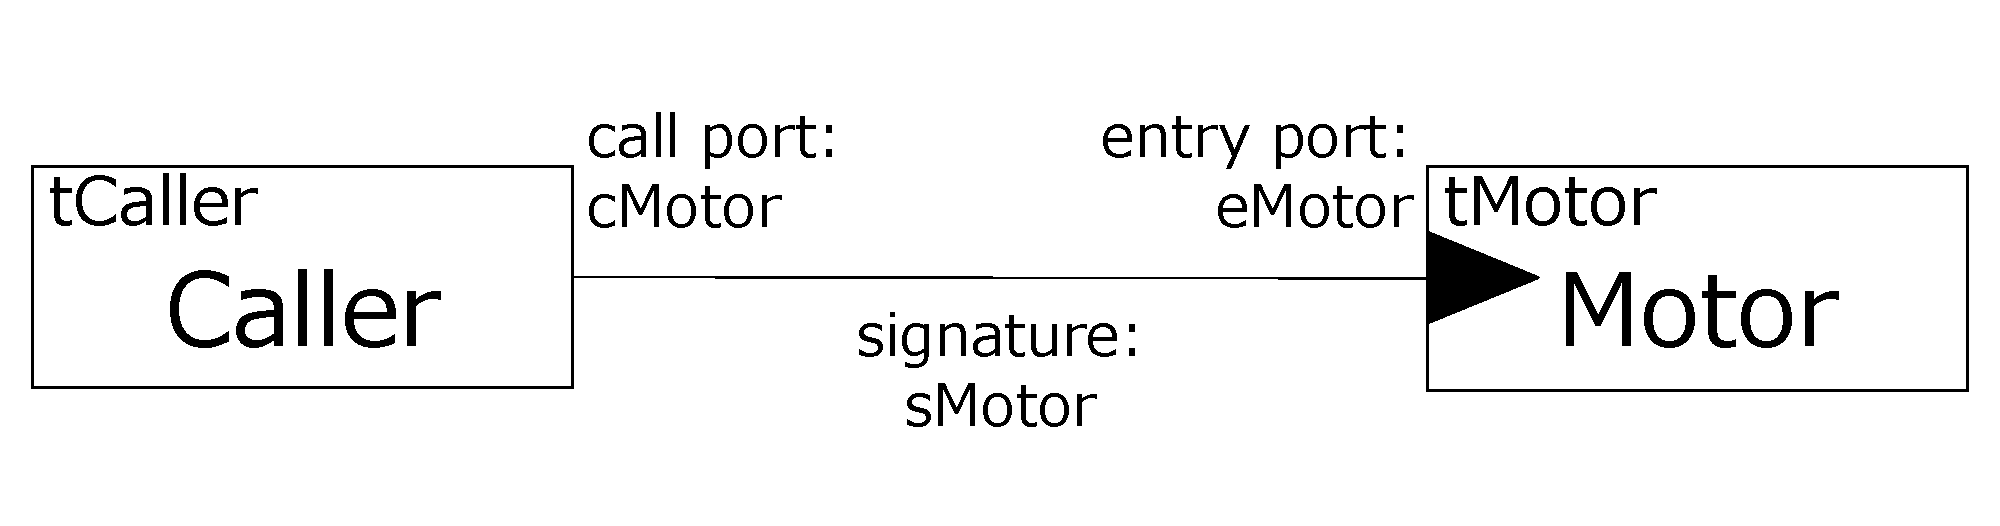
\includegraphics[width=8cm,clip]{../EMSOFT2016/figure/component_diagram.pdf}
    \caption{TECSコンポーネント図の例}
    \vspace{-2mm}
    \label{fig:component}
\end{figure}

\subsubsection{コンポーネント記述}
TECSのコンポーネント記述は,シグニチャ記述,セルタイプ記述,組上げ記述の3つに分類され,.cdlファイルに記述する.
図\ref{fig:component}に示されるコンポーネント記述について次に述べる.

% \begin{description}
%     \item[{\bf シグニチャ記述}]\mbox{}\\
        シグニチャ記述は,セルのインタフェースを定義する.
        図\ref{signature}に示す通り,{\it signature}キーワードに続けて,シグニチャ名(sMotor)を記述する.
        %図\ref{signature}のようにシグニチャsMotorを定義できる.
        TECSでは,インタフェースの定義を明確にするために,入力と出力にはそれぞれ,[in]と[out]という指定子がつけられる.
        
\begin{figure}[t]
\centering
\begin{lstlisting}
signature sMotor{
    int32_t getCounts( void );
    ER resetCounts( void );
    ER setPower( [in]int power );
    ER stop( [in] bool_t brake );
    ER rotate( [in] int degrees, [in] uint32_t speed_abs,
              [in] bool_t blocking );
    void initializePort( [in]int32_t type );
};
\end{lstlisting}
\caption{シグニチャ記述}
\vspace{-2mm}
\label{signature}
\end{figure}

    % \item[{\bf セルタイプ記述}]\mbox{}\\
        セルタイプ記述は,受け口,呼び口,属性,変数を用いてセルタイプを定義する.
        {\it celltype}キーワードに続けて,セルタイプ名(tCaller)を記述する.
        図\ref{celltype}に示す通り,受け口は,{\it entry}キーワードに続けて,シグニチャ名, 受け口名を記述する.
        同様にして,呼び口も定義できる.
        属性と変数は,それぞれ{\it attr},{\it var}キーワードを用いて列挙する.

\begin{figure}[t]
\centering
\begin{lstlisting}
celltype tCaller{
    call sMotor cMotor;
};
celltype tMotor{
    entry sMotor eMotor;
    attr{ int32_t attr = 100; };
    var{ int32_t var; };
};
\end{lstlisting}
\caption{セルタイプ記述}  
\vspace{-2mm}
\label{celltype}
\end{figure}

    % \item[{\bf 組上げ記述}]\mbox{}\\
        組上げ記述は,セルをインスタンス化し,セルを結合する.
        {\it cell}キーワードに続けて,セルタイプ名,セル名を記述する.
        呼び口名,``=",結合先の受け口名の順に記述し,セルを結合する.
        図\ref{build}では,セルCallerの呼び口cMotorと,セルMotorの受け口eMotorが接続されている.
        
\begin{figure}[t]
\centering
\begin{lstlisting}
cell tMotor Motor{
};
cell tCaller Caller{
    cMotor = Motor.eMotor;
};
\end{lstlisting}
\caption{組上げ記述}
\vspace{-2mm}
\label{build}
\end{figure}

% \end{description}
\vspace{-3mm} 
\subsection{mruby on TECS}
\label{sec:mruby on TECS}
mruby on TECSは,mruby(軽量Ruby)を用いた組込みソフトウェアのコンポーネントベース開発が可能なフレームワークである.

\subsubsection{システムモデル}
%図\ref{fig:mrubyontecs}にmruby on TECSのシステムモデルを示す.
mrubyバイトコードはそれぞれ,コンポーネント化されたRTOSのタスクとして,RiteVM上で実行される.
%TECSのコンポーネントは,モータドライバやセンサドライバのような組込みドライバをサポートしている.

mruby-TECSブリッジによって,mrubyプログラムからC言語の関数を呼び出すことができる.
%mruby-TECSブリッジについては,以下で詳しく説明する.

本研究では,RTOSとして,TOPPERS/HRP2\cite{par:hr-tecs}を使用した.
TOPPERS/HRP2は,$\mu$ITRON\cite{par:microITRON}をベースにしたメモリ保護機能を持つRTOSである.
しかし,TECSは,TOPPERS/HRP2だけでなく,OSEK\cite{par:OSEK}やTOPPERS/ASP\cite{url:ASP}といったRTOSにも対応しているため,mruby on TECSはRTOSに依存しない.

% \begin{figure}[t]
%     \centering
%     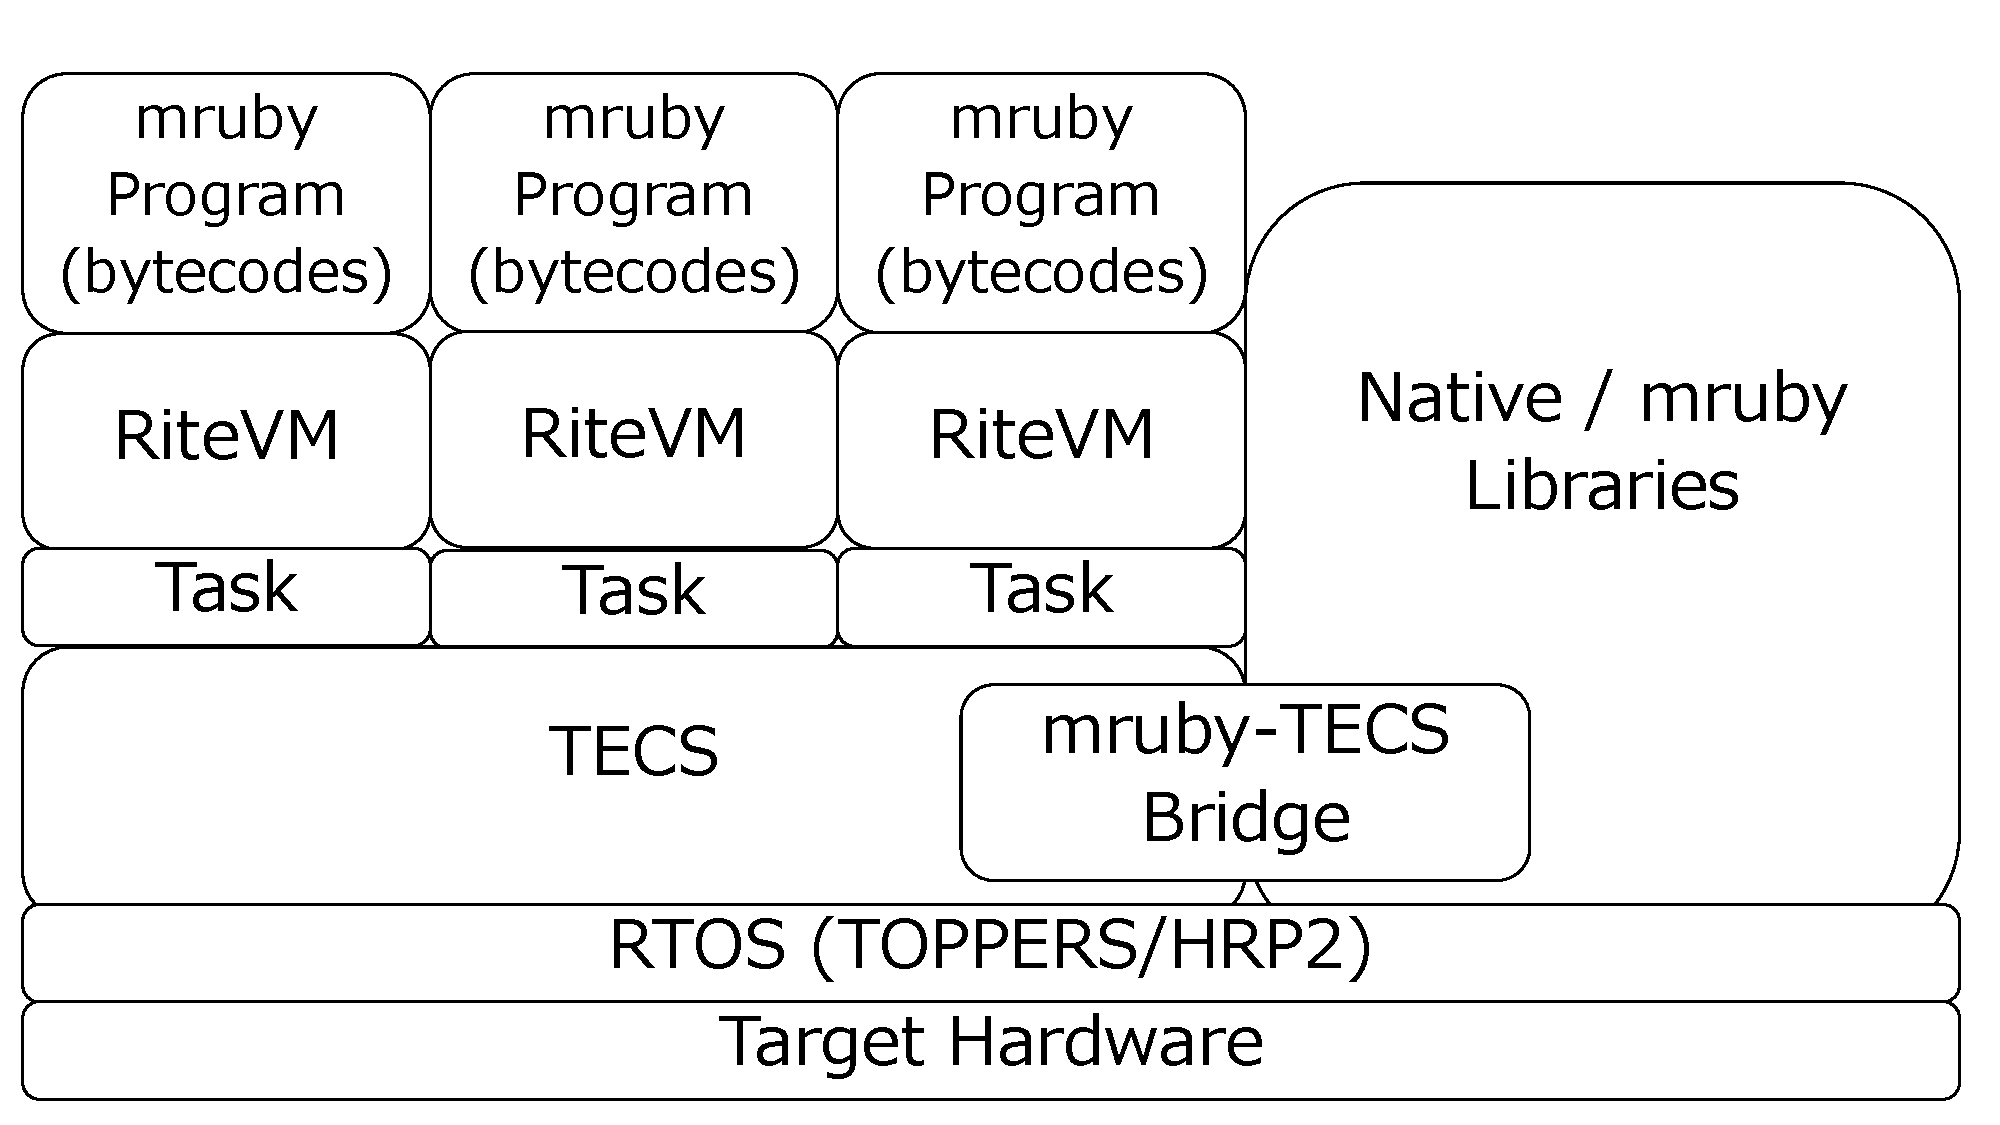
\includegraphics[width=8cm,clip]{../EMSOFT2016/figure/mrubyontecs.pdf}
%     \caption{System Model of existing mruby on TECS}
%     \label{fig:mrubyontecs}
% \end{figure}

% \subsubsection{mruby-TECSブリッジ}
% mrubyとC言語には,実行時間に大きな差がある.
% \cite{par:mrubyonTECS}によると, mrubyプログラムは,C言語より実行時間が数百倍遅い.
% これによって,mrubyプログラムをすべてアプリケーションに使用することは難しい.
% mrubyを使用することにより,生産性やメンテナンス性を向上させることができる一方で,アクチュエータやセンサを制御するようなアプリケーションの重要な部分をC言語で実装することも必要である.
%
% 図\ref{fig:mruby_TECS_bridge}に,モータ制御に対するmruby-TECSブリッジの例を示す.
% BridgeMotorの左部分は,mrubyプログラムであり,右部分は,TECSのコンポーネントである.
% \begin{figure}[t]
%     \centering
%     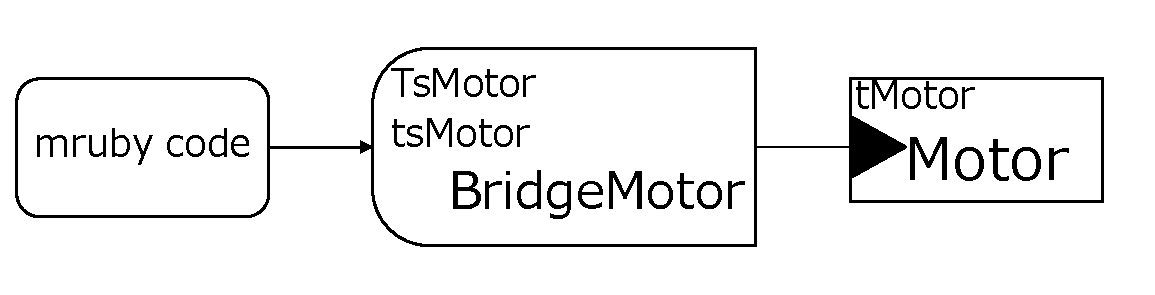
\includegraphics[width=8cm,clip]{../EMSOFT2016/figure/mruby_TECS_bridge.pdf}
%     \caption{mruby-TECS Bridge}
%     \label{fig:mruby_TECS_bridge}
% \end{figure}
%
% mruby-TECSブリッジは,mrubyプログラムからの呼び出しを受け取るためのセルタイプと,C関数を呼び出すためのmrubyクラスを生成する.
% 生成されたmruby-TECSブリッジのコードがmrubyのクラスとメソッドを登録する.
% これによって,mrubyプログラムからあるメソッドが呼ばれると,mruby-TECSブリッジがTECSコンポーネントで定義されたC関数を呼び出す.
%
\section{設計と実装}
\vspace{-2mm}
\label{sec:Design and Implementation}
図\ref{fig:system_model}に提案フレームワークの詳細なシステムモデルを示す.
ホストから転送されたmrubyアプリケーションのバイトコードは,それぞれのRiteVMに実装されたローダで受信され,同期処理され実行される.
RiteVMスケジューラはタスクを周期的に切り替えるため,mrubyアプリケーションは並行動作できる.
また,mrubyアプリケーションの起動は同期機構により同期される. 
\begin{figure}[t]
    \centering
    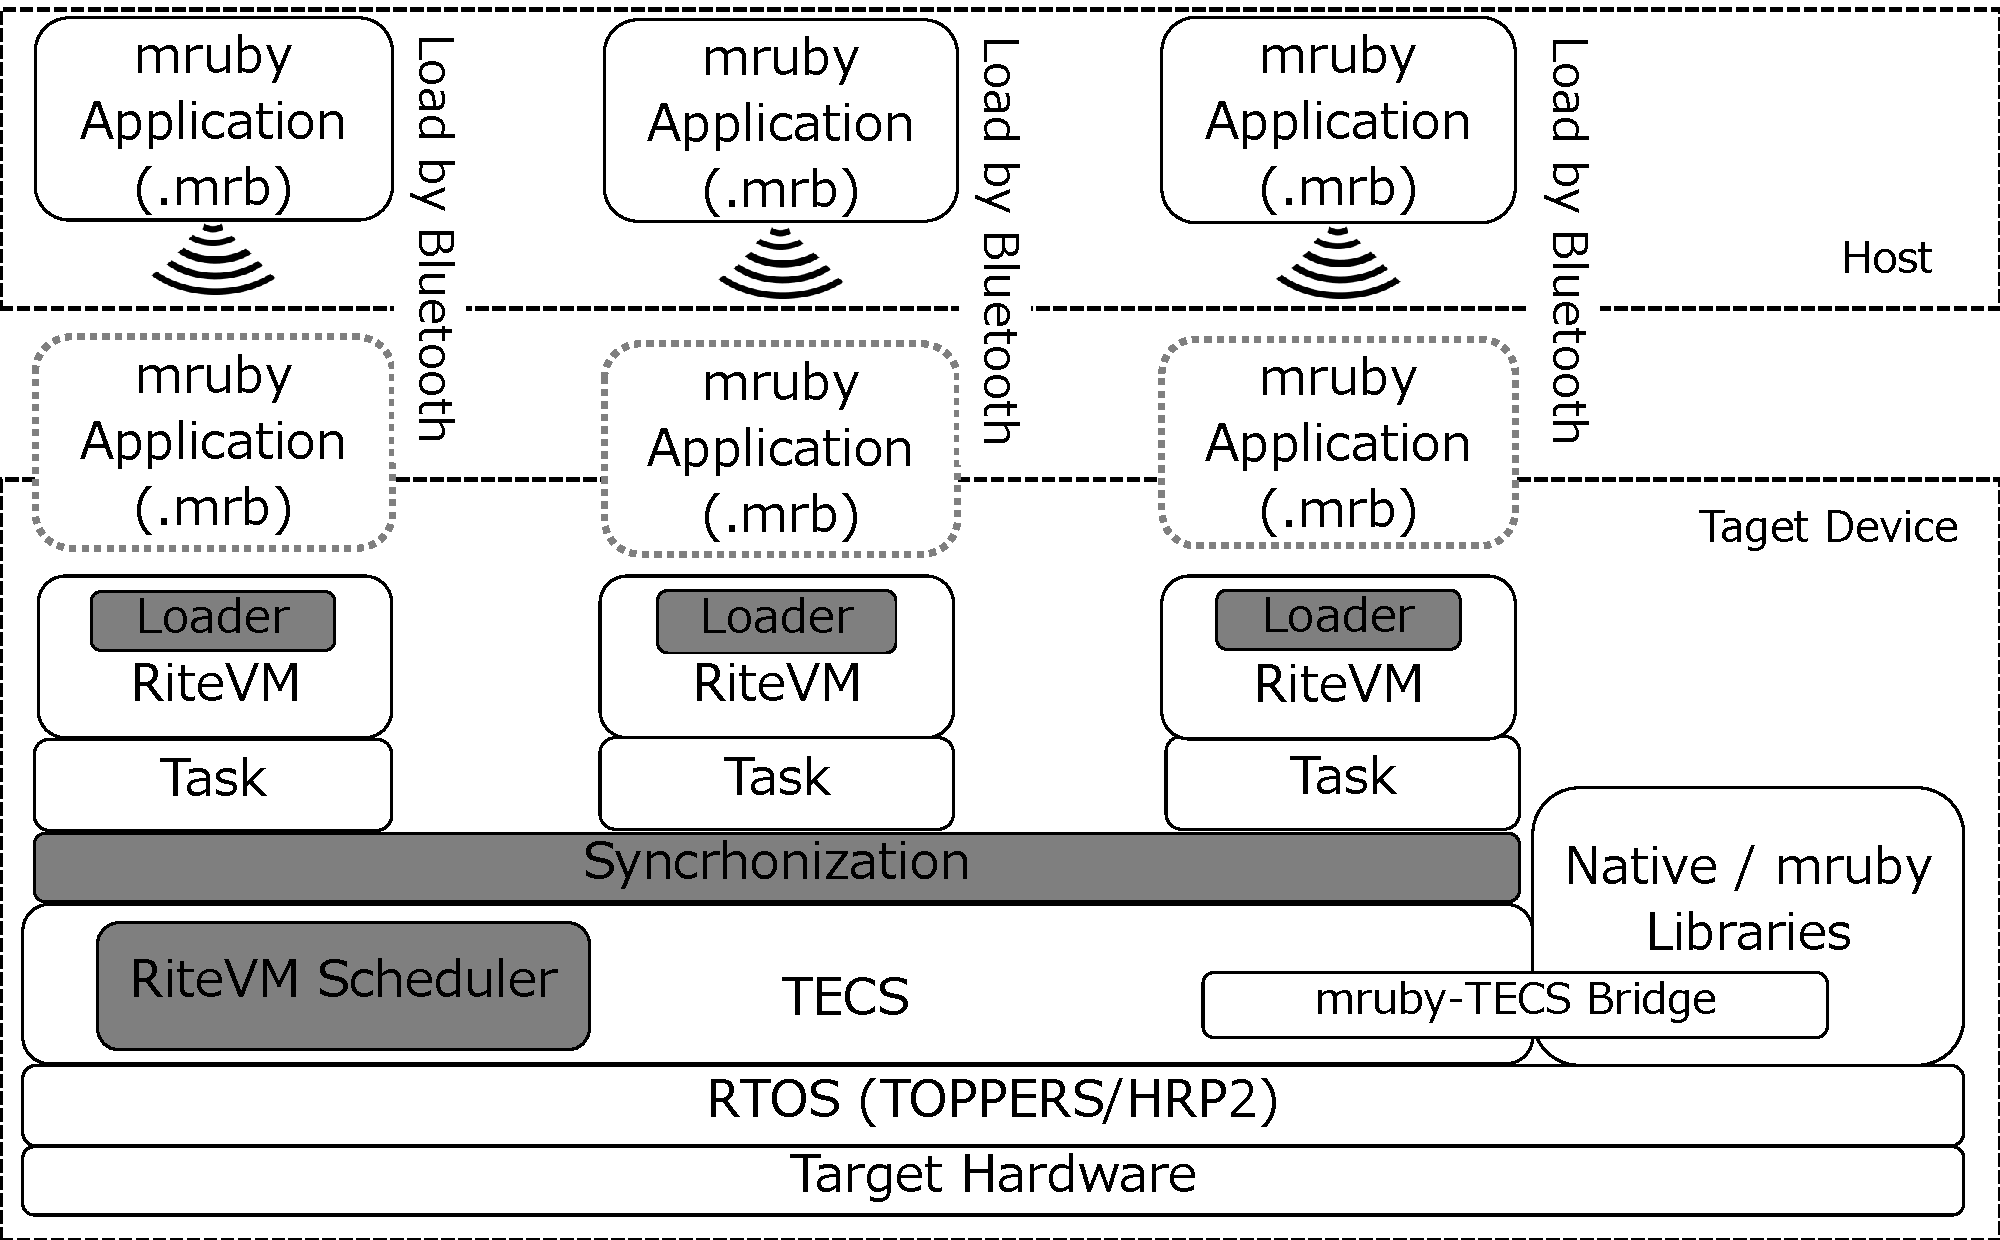
\includegraphics[width=8cm,clip]{../EMSOFT2016/figure/system_model.pdf}
    \caption{提案フレームワークの詳細なシステムモデル}
\vspace{-2mm}
    \label{fig:system_model}
\end{figure}

\subsection{Bluetoothを用いたmrubyバイトコードローダ}
\label{sec:mruby bytecode loader using Bluetooth}
この章では,Bluetoothを用いたmrubyバイトコードローダについて述べる.
既存フレームワークでは,mrubyバイトコードをプラットフォームに組み込んでいるため,mrubyプログラムを修正する度にプラットフォーム部分をもう一度コンパイル・リンクし,SDカードやROMに再度書き込み,OSを再起動する必要がある.
%このような作業を繰り返すことで,作業効率は悪くなる.
提案フレームワークでは,一度だけSDカードやROMに書き込むため,作業効率を向上できる.

mrubyプログラムは,アプリケーション部分とライブラリ部分に分けられる.
mrubyアプリケーションは,開発者が主にプログラムするメインのコードであり,mrubyライブラリには,motorクラスやsensorクラスといったRubyクラスのようにアプリケーションで利用される関数群が定義されている.
アプリケーションとライブラリを含んだmrubyバイトコードを転送し,実行することもできるが,提案フレームワークでは,ライブラリ部分はプラットフォームに組み込み,アプリケーション部分のみを転送する設計にした.
この設計にすることで,転送するバイトコードのサイズや処理時間の無駄を省ける.
さらに,各RiteVMでライブラリを共有することや,固有のライブラリを持つことも可能になる.

提案フレームワークでは,mrubyバイトコードの連続ローディングにも対応している.

\subsubsection{ローダを実装したRiteVMのコンポーネント}
ローダを実装したRiteVMはTECSのコンポーネントとして提供されている.
このコンポーネントは,RiteVMのコンポーネント\cite{par:mrubyonTECS}の拡張である.
このコンポーネントでは,転送されたバイトコードの受信に加え,RiteVMのコンフィグレーションが行われる.

図\ref{fig:component_bluetooth}に,MrubyTask1とMrubyBluetooth1のコンポーネントの例を示す.
MrubyTask1は,コンポーネント化されたRTOS (TOPPERS/HRP2\cite{par:hr-tecs})のタスクである.
MrubyBluetooth1は,ローダを実装したRiteVMのコンポーネントであり,転送されるバイトコードを受信する.
提案フレームワークでは,バイナリ転送プロトコルとして,ZMODEMを適用した.

\begin{figure}[t]
    \centering
    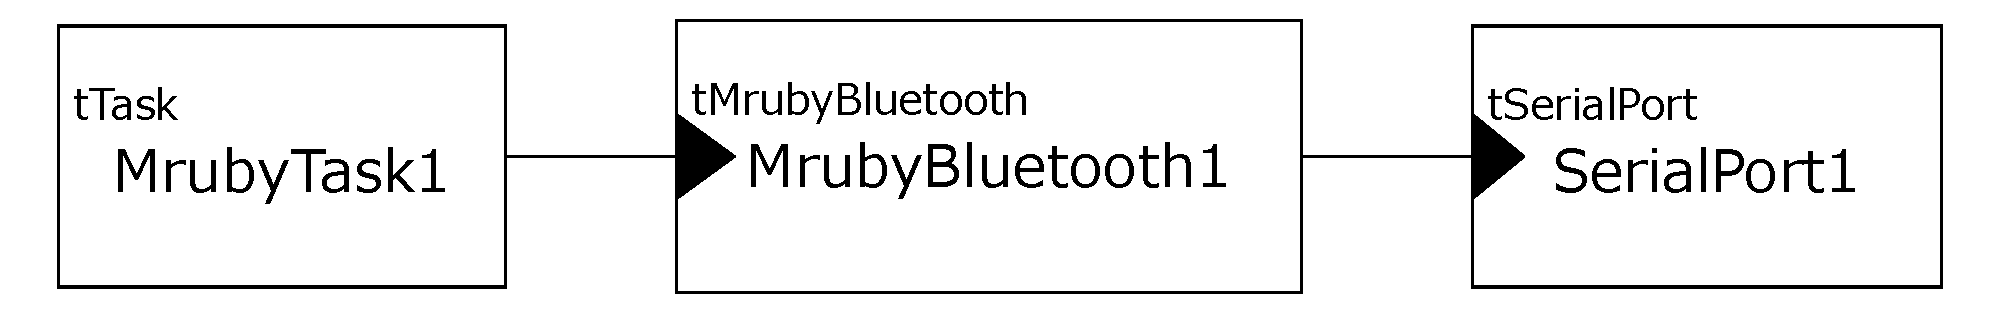
\includegraphics[width=8cm,clip]{../EMSOFT2016/figure/component_bluetooth.pdf}
    \caption{ローダを実装したRiteVMのコンポーネント図}
\vspace{-2mm}
    \label{fig:component_bluetooth}
\end{figure}

図\ref{fig:control_flow}に,ローダを実装したRiteVMがmrubyプログラムを実行するまでのフローチャート,図\ref{maincode_mrubybluetooth}には,RiteVMコンポーネントのソースコードを示す.

はじめに,mrubyで使われる状態と変数のセットである{\it mrb\_state}と{\it mrbc\_context}のポインタを初期化する.
%{\it mrb\_state}は,mrubyで使われる状態と変数のセットである.

次に,mrubyライブラリのバイトコードを読み込む.
図\ref{celltype_mrubybluetooth}に示すように,tMrubyBluetoothのセルは属性を持っている.
{\it mrubyFile}はmrubyライブラリのファイルを示しており,{\it [omit]}はTECSジェネレータによってのみ使われるため,この属性はメモリを消費しない.
{\it irep}は,mrubyライブラリのバイトコードが格納されている配列へのポインタである.
つまり,mrubyライブラリは始めのコンパイル時にコンポーネントの属性として,配列に保存される.

次に,転送されてきたmrubyアプリケーションのバイトコードを読み込む.
mrubyアプリケーションのバイトコードは,図\ref{celltype_mrubybluetooth}に示す,変数uint8\_t型の配列{\it irepApp}に格納される.
2つのバイトコードは,それぞれ別の配列に保存されており,別々に読み込まれる.

最後に,RiteVMはmrubyアプリケーションであるタスクを実行する.
mrubyアプリケーションのプログラムが修正された場合は,そのバイトコードのみを再転送する.

\begin{figure}[t]
    \centering
    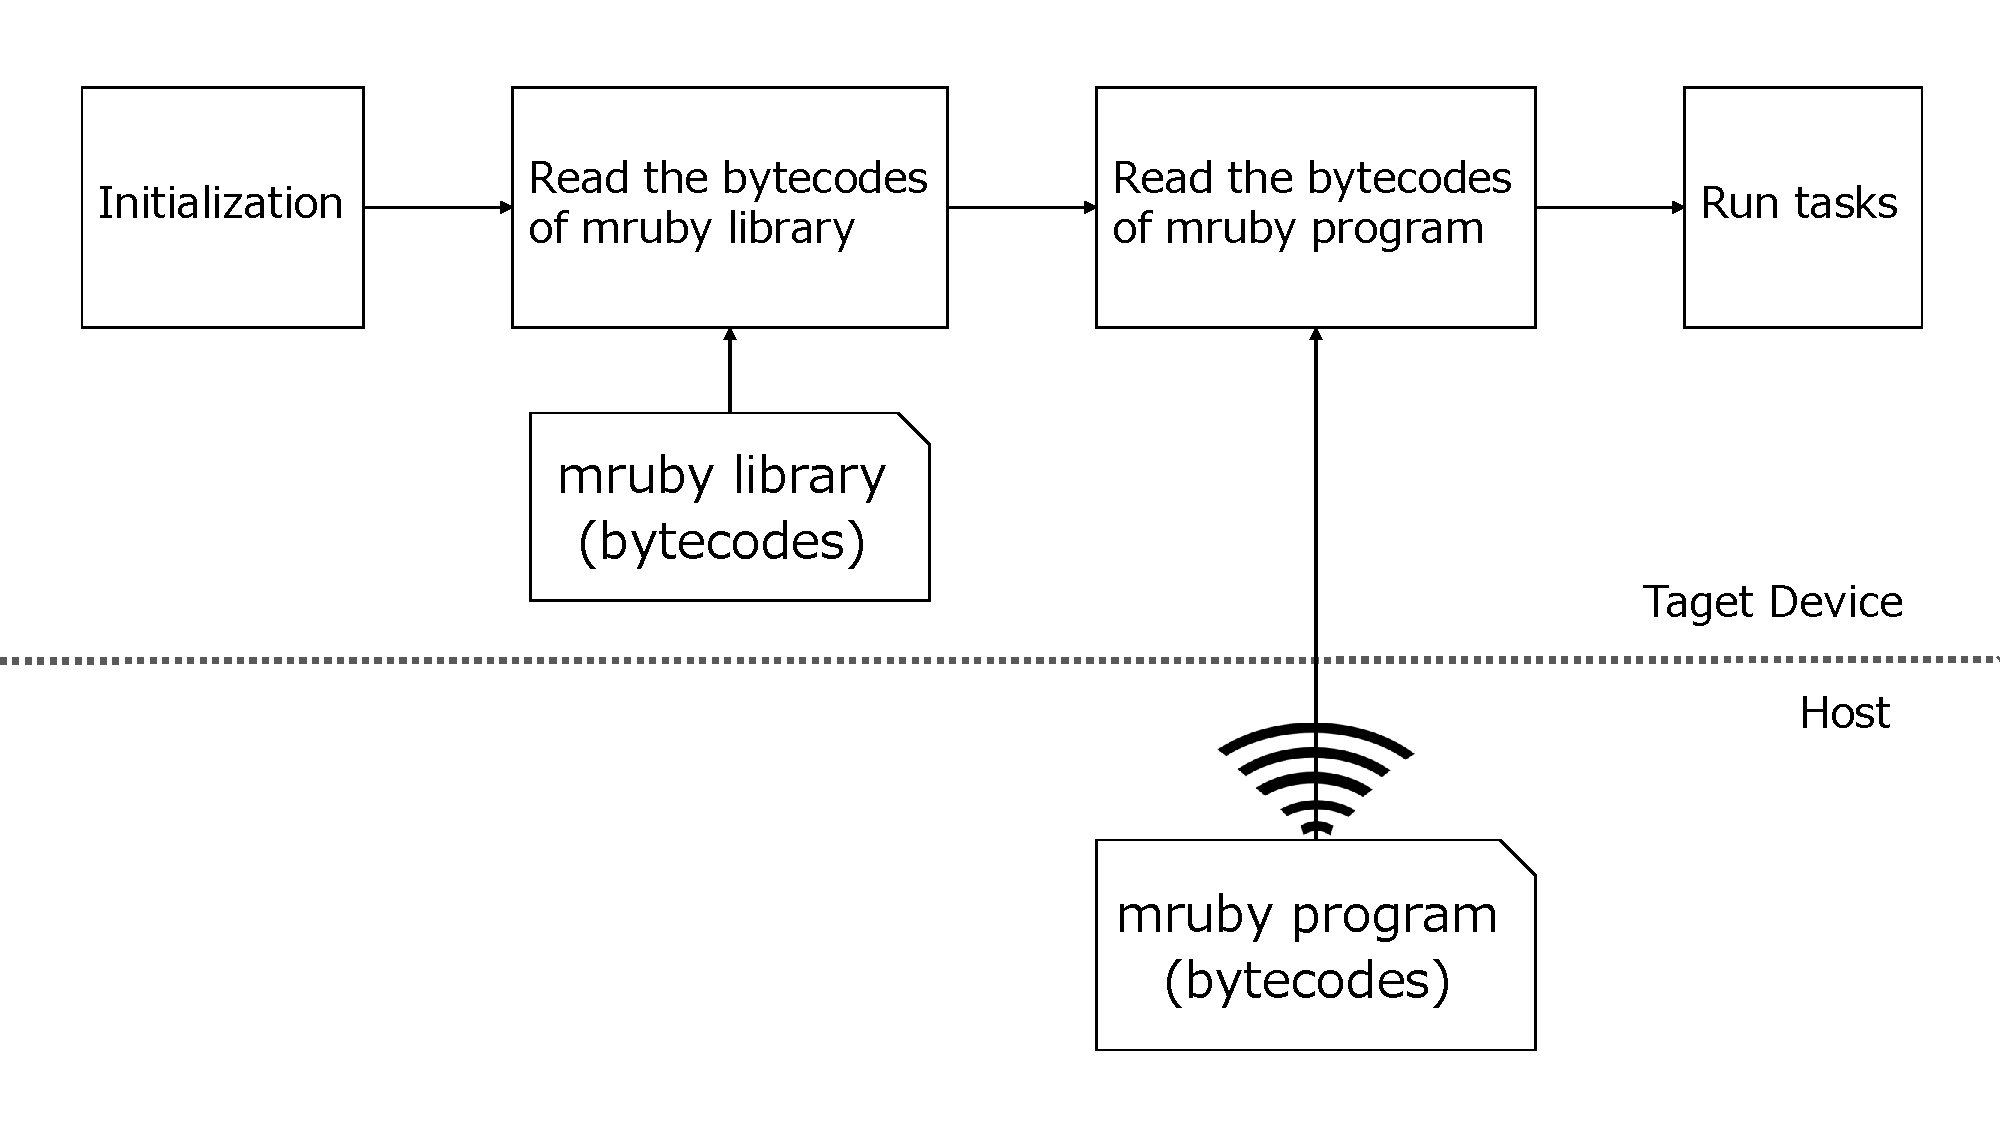
\includegraphics[width=8cm,clip]{../EMSOFT2016/figure/control_flow.pdf}
    \caption{ローダの処理フローチャート}
\vspace{-2mm}
    \label{fig:control_flow}
\end{figure}
\begin{figure}[t]
\centering
\begin{lstlisting}
celltype tMrubyBluetooth{
  entry sTaskBody eMrubyBody;
  attr{
    [omit]char_t *mrubyFile;
    char_t *irep = C_EXP("&$cell_global$_irep");
    uint32_t irepAppSize = C_EXP( BUFFER_SIZE );
  };
  var{ [size_is(irepAppSize)] uint8_t *irepApp; };
};
\end{lstlisting}
\caption{ローダを実装したRiteVMのセルタイプ記述}
\label{celltype_mrubybluetooth}
\end{figure}
\begin{figure}[t]
\centering
\begin{lstlisting}
void eMrubyBody_main( CELLIDX idx ){
  /*Omit: Declaration variables*/
  mrb=mrb_open(); /*New interpreter instance*/
  /*Omit: error check for mrb_state*/
  c=mrbc_context_new( mrb ); /*New mruby context*/
  /*Omit: initialization of mruby-TECS bridge*/
  /*Receive the bytecode via Bluetooth*/
  bluetooth_loader( VAR_irepApp );
  /*Load mruby library bytecode and run*/
  mrb_load_irep_cxt( mrb, ATTR_irep, c );
  /*Load mruby application bytecode and run*/
  mrb_load_irep_cxt( mrb, VAR_irepApp, c );
  mrbc_context_free( mrb, c ); /*Free mruby context*/
  mrb_close( mrb ); /*Free interpreter instance*/
}

\end{lstlisting}
\caption{ローダを実装したRiteVMのメインコード}
\vspace{-2mm}
\label{maincode_mrubybluetooth}
\end{figure}
\subsection{マルチタスク処理}
\label{sec:Multitask}
この章では,提案フレームワークでのマルチタスク処理の設計について述べる.
%mruby on TECSは,マルチタスクに対応しているが,開発者がRTOSの知識を熟知している必要がある.

マルチタスク処理のアプローチのひとつにコルーチンがある.
コルーチンは,協調的スレッドであり,開発者が{\it resume}や{\it yield}といった関数を呼び出すことで並列動作できるが,ノンプリエンプティブな処理で,開発者自身がタスクの切り替えを行う必要があるので,OSのサポートやマルチコアの恩恵を受けることができない.
Rubyのコルーチンは,Fiberクラス\cite{url:co-routine}に定義されている.

その他にも,$\mu$ITRONのサービスコールである{\it delay()}を使った手法がある.
このサービスコールは,引数として与えられた時間だけ,そのタスクの起動を遅らせる.
{\it delay()}は,固定優先度スケジューリングの場合に用いられるが,フェアスケジューリングの場合には使用することが難しい.

提案フレームワークでは,フェアスケジューラであるRiteVMスケジューラを実装し,複数のタスクを平等に並行動作させる.
このスケジューラはアプリケーションタスクが同じ優先度を持つ場合に利用でき,開発者がOSの関数を呼び出すことなく,マルチタスク処理が可能になる.
その上,既存のアプリケーションプログラムの構造を変えることなく使うことができる. 

\subsubsection{RiteVMスケジューラ}
RiteVMスケジューラは,周期ハンドラであり,同優先度のタスクの実行を切り替える$\mu$ITRONのサービスコールである{\it rotateReadyQueue}を周期的に呼び出す.
%{\it rotateReadyQueue}は,同優先度のタスクの実行を切り替える関数である.
RiteVMスケジューラの設計を図\ref{fig:rotateReadyQueue}に示す.

% 無限ループを持った同優先度の2つのタスクの場合を考える.
% 現状のシステムでは,始めにタスクが起動すると,そのタスクが無限ループに入るため,もう片方のタスクが起動することができない.

{\it rotateReadyQueue}が呼ばれると,図\ref{fig:rotateReadyQueue}に示すように,タスクの起動が切り替わる.
{\it rotateReadyQueue}の引数は,優先度である.

{\it rotateReadyQueue}は,2つ以上のタスクの場合にでも利用できる.
例えば,3つのタスク,task 1, 2, 3が順に起動する場合,{\it rotateReadyQueue}が呼ばれると,task 2, 3, 1の順にタスクの起動は切り替わる.

\begin{figure}[t]
    \centering
    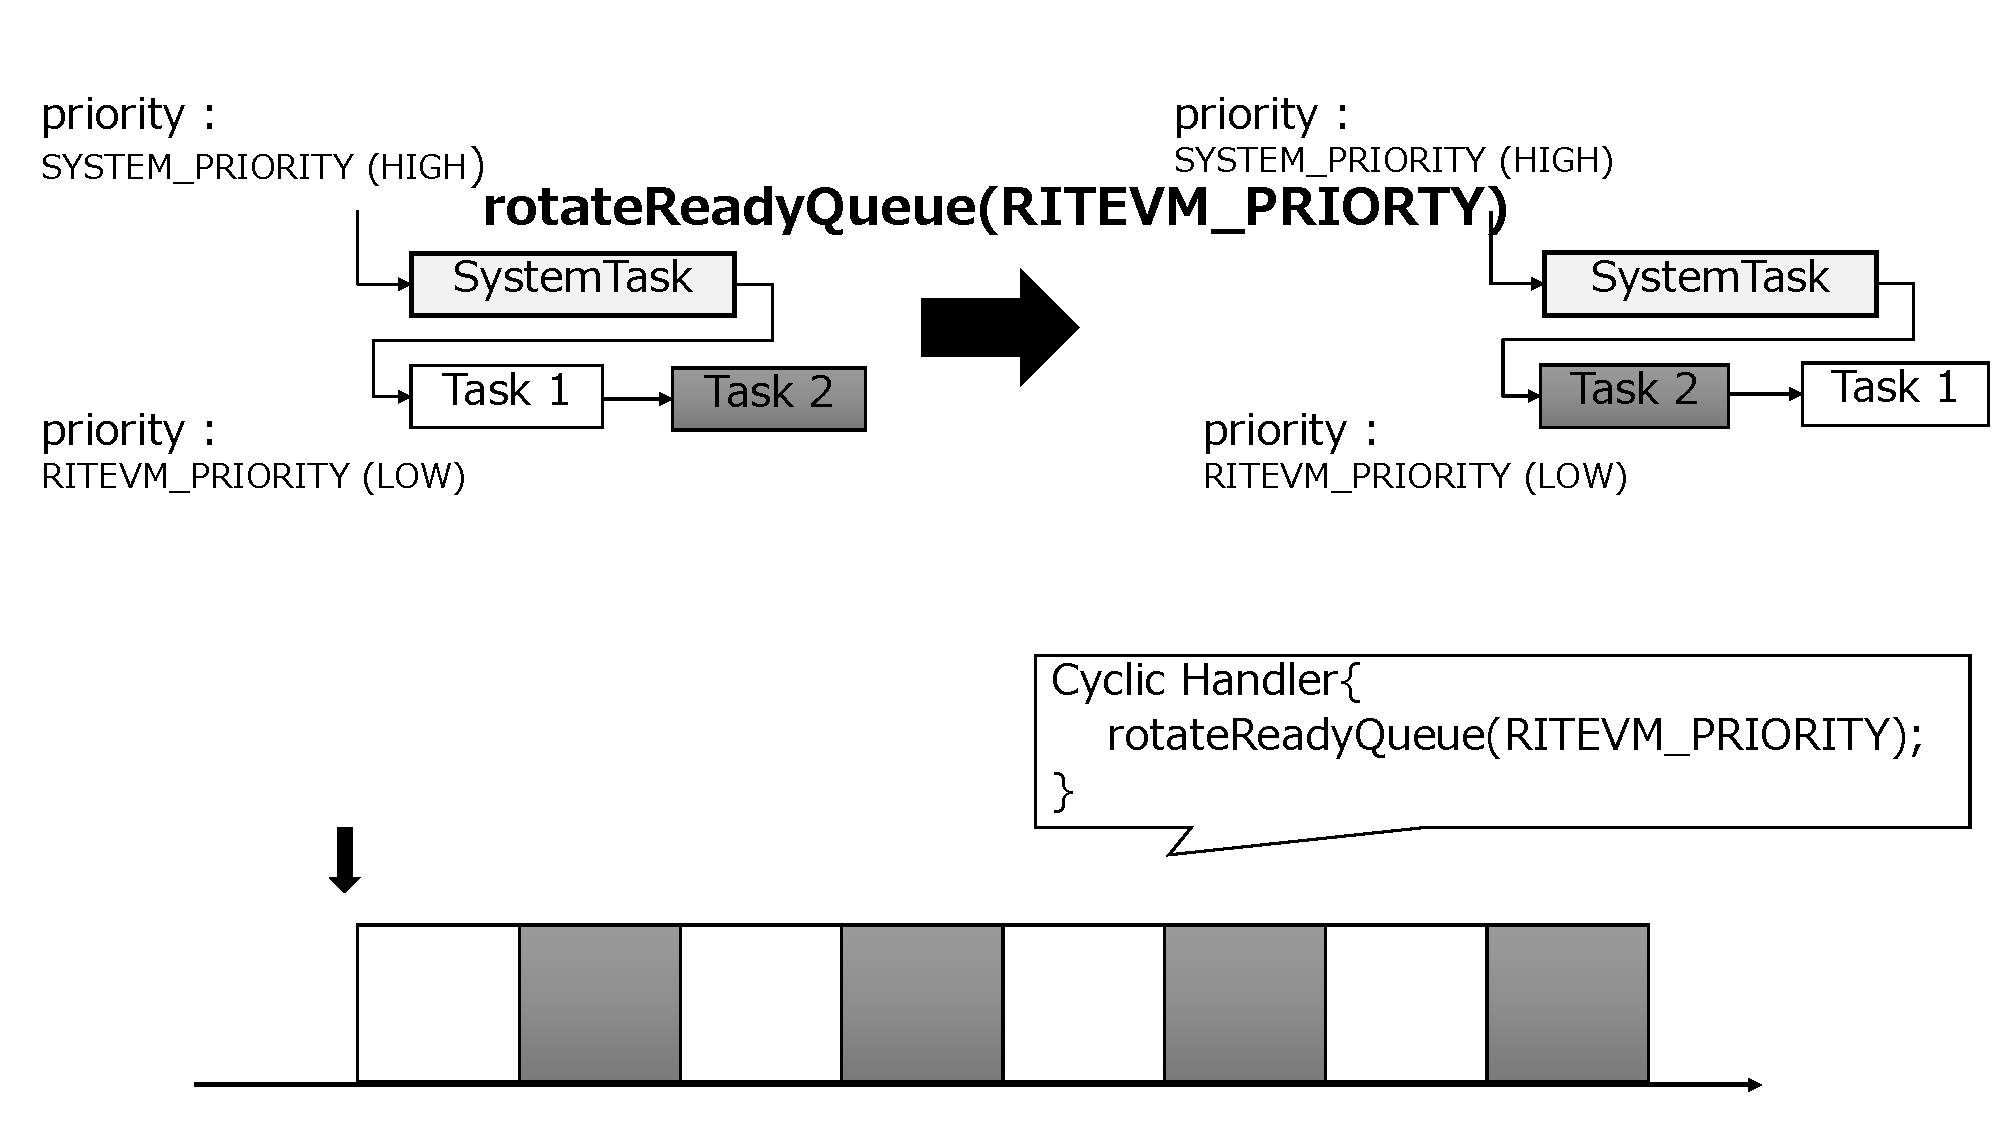
\includegraphics[width=8cm,clip]{../EMSOFT2016/figure/rotateReadyQueue.pdf}
    \caption{RiteVMスケジューラの設計}
\vspace{-2mm}
    \label{fig:rotateReadyQueue}
\end{figure} 
 
\subsubsection{RiteVMスケジューラのコンポーネント}
%図\ref{fig:cyclic_handler}にRiteVMスケジューラのコンポーネント図を示す.
RiteVMスケジューラのコンポーネントは,CyclicHandlerとCyclicMainから構成される.
CyclicHandlerセルは,$\mu$ITRONの周期ハンドラの設定を行う.
$\mu$ITRONの周期ハンドラは,\cite{par:microITRON}に詳しく書かれている.

周期ハンドラは,5つの引数(ID, attribute, cyclic time, cyclic phase, access pattern)を持っている.
CyclicHandlerセルは,3つの引数をセルの属性として持っている.
CyclicMainセルは,周期ハンドラの処理を行うコンポーネントであり,{\it rotateReadyQueue}が実装されている.
%図\ref{celltype_cyclic_handler}に,セルタイプtCyclicMainのセルタイプ記述を示す.
呼び口は,カーネルの機能である{\it rotateReadyQueue}を使用するためにカーネルセルの受け口({\it tkernel.eiKernel})に接続されている.
属性は,{\it rotateReadyQueue}の引数として使われる.

%図\ref{build_cyclic_handler}に,図\ref{fig:cyclic_handler}に示されるコンポーネントの組上げ記述を示す.
図\ref{build_cyclic_handler}に,RiteVMスケジューラのコンポーネント組上げ記述を示す.
CyclicHandlerセル部分では,cyclicTimeやcyclicPhaseといった属性で与えられる周期ハンドラの設定を行う.
attributeは,OSの起動とすると実行状態になる{\it TA\_STA}が与えられる.
周期時間は,1msecである.
CyclicMainセル部分には,属性としてpriorityが記述されている.
RITEVM\_PRIORITYはmrubyタスクの優先度を定義しており,{\it rotateReadyQueue}の引数として与えられる.

% \begin{figure}[t]
%     \centering
%     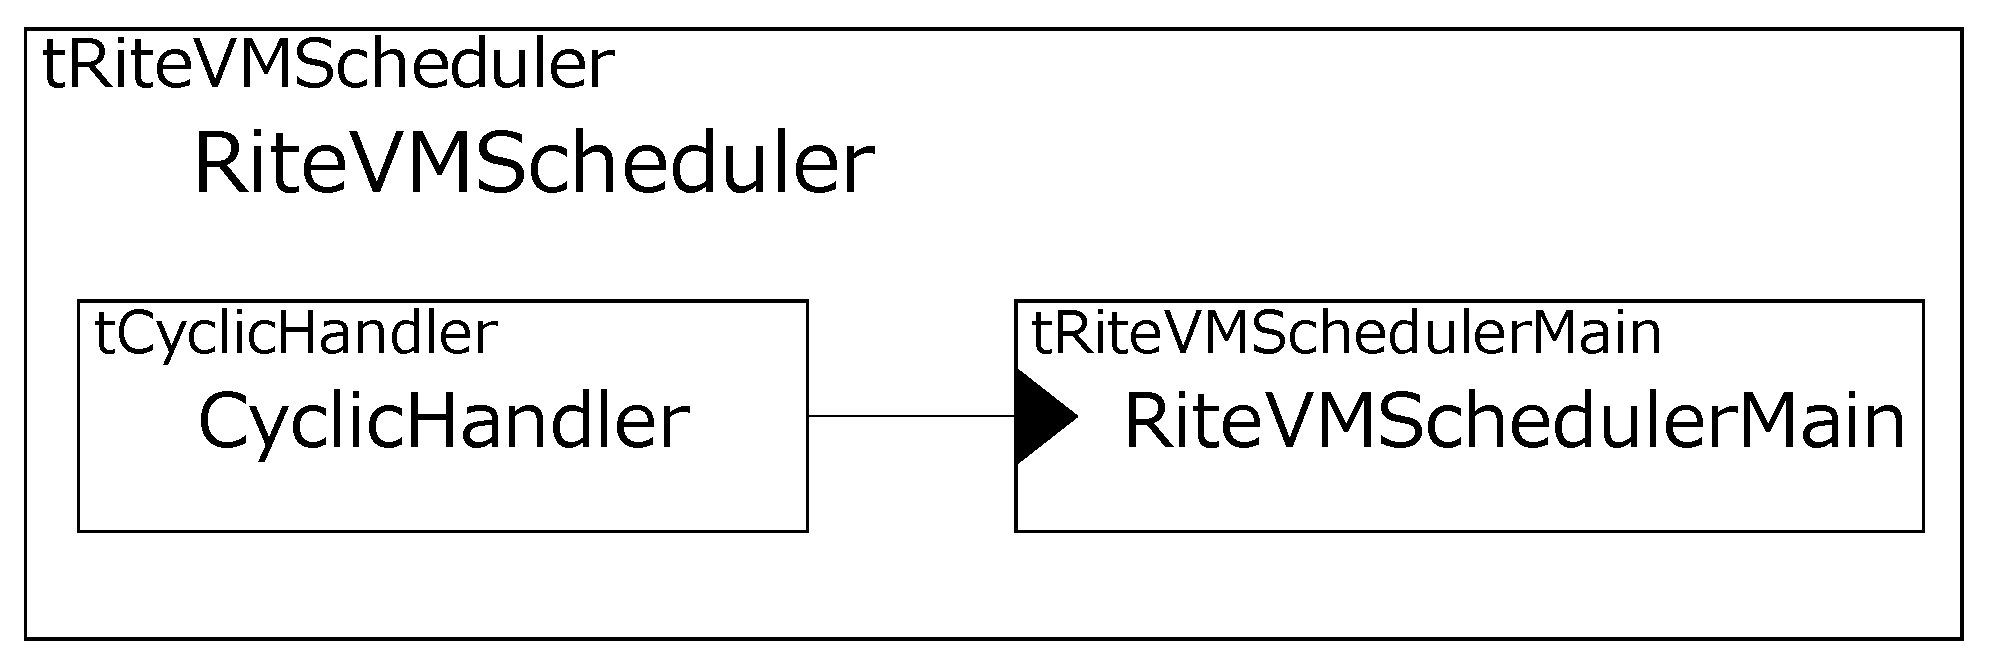
\includegraphics[width=8cm,clip]{../EMSOFT2016/figure/cyclic_handler.pdf}
%     \caption{Component Diagram of Cyclic Handler}
%     \label{fig:cyclic_handler}
% \end{figure}
% \begin{figure}[t]
%     \centering
%     \begin{lstlisting}
% celltype tCyclicHandler {
%     [inline] entry sCyclic eCyclic;
%     call  siHandlerBody  ciBody;
%     attr {
%     	[omit] ATR    attribute = C_EXP("TA_NULL");
%     	[omit] RELTIM cyclicTime;
%     	[omit] RELTIM cyclicPhase = 0;
%     };
% };
% celltype tCyclicMain{
%     require tKernel.eiKernel;
%     entry siHandlerBody eiBody;
%     attr {
%         PRI priority;
%     };
% };
%     \end{lstlisting}
%     \caption{Celltype Description of Cyclic Handler}
%     \label{celltype_cyclic_handler}
% \end{figure}
\begin{figure}[t]
    \centering
    \begin{lstlisting}
cell tCyclicHandler CyclicHandler{
    ciBody = CyclicMain.eiBody;
    attribute = C_EXP("TA_STA");
    cyclicTime = 1;
    cyclicPhase = 1;
};
cell tCyclicMain CyclicMain{
    priority = C_EXP("RITEVM_PRIORITY");
};
   \end{lstlisting}
    \caption{RiteVMスケジューラの組上げ記述}
\vspace{-2mm}
    \label{build_cyclic_handler}
\end{figure}
 
\subsubsection{mrubyアプリケーションの同期機構}
複数のmrubyアプリケーションの起動を同期させるために,イベントフラグを適用した.
タスクはそれぞれ0x01(01),0x02(10)のパターンをセットし,待ちパターン0x3(11)でAND待ちする.
この機構は,2つ以上のタスクの場合でも適用できる.
例えば,タスクが4つの場合,タスクはそれぞれ,0x01(0001), 0x02(0010), 0x04(0100), 0x08(1000)のパターンをセットし,待ちパターン0x0f(1111) でAND待ちする.(図\ref{fig:Eventflag} (A))

さらに,提案フレームワークでは,バイトコードの連続ローディングに対応するため,アプリケーションの終了も同期を行う.
これによって,すぐに終了するようなアプリケーションのRiteVMが,次のロードの待機状態に入るのを防ぐことができる.
すべてのアプリケーションは同時に終了し,すべてのRiteVMは同時に次のロードの待機状態になる.

\begin{figure}[t]
    \centering
    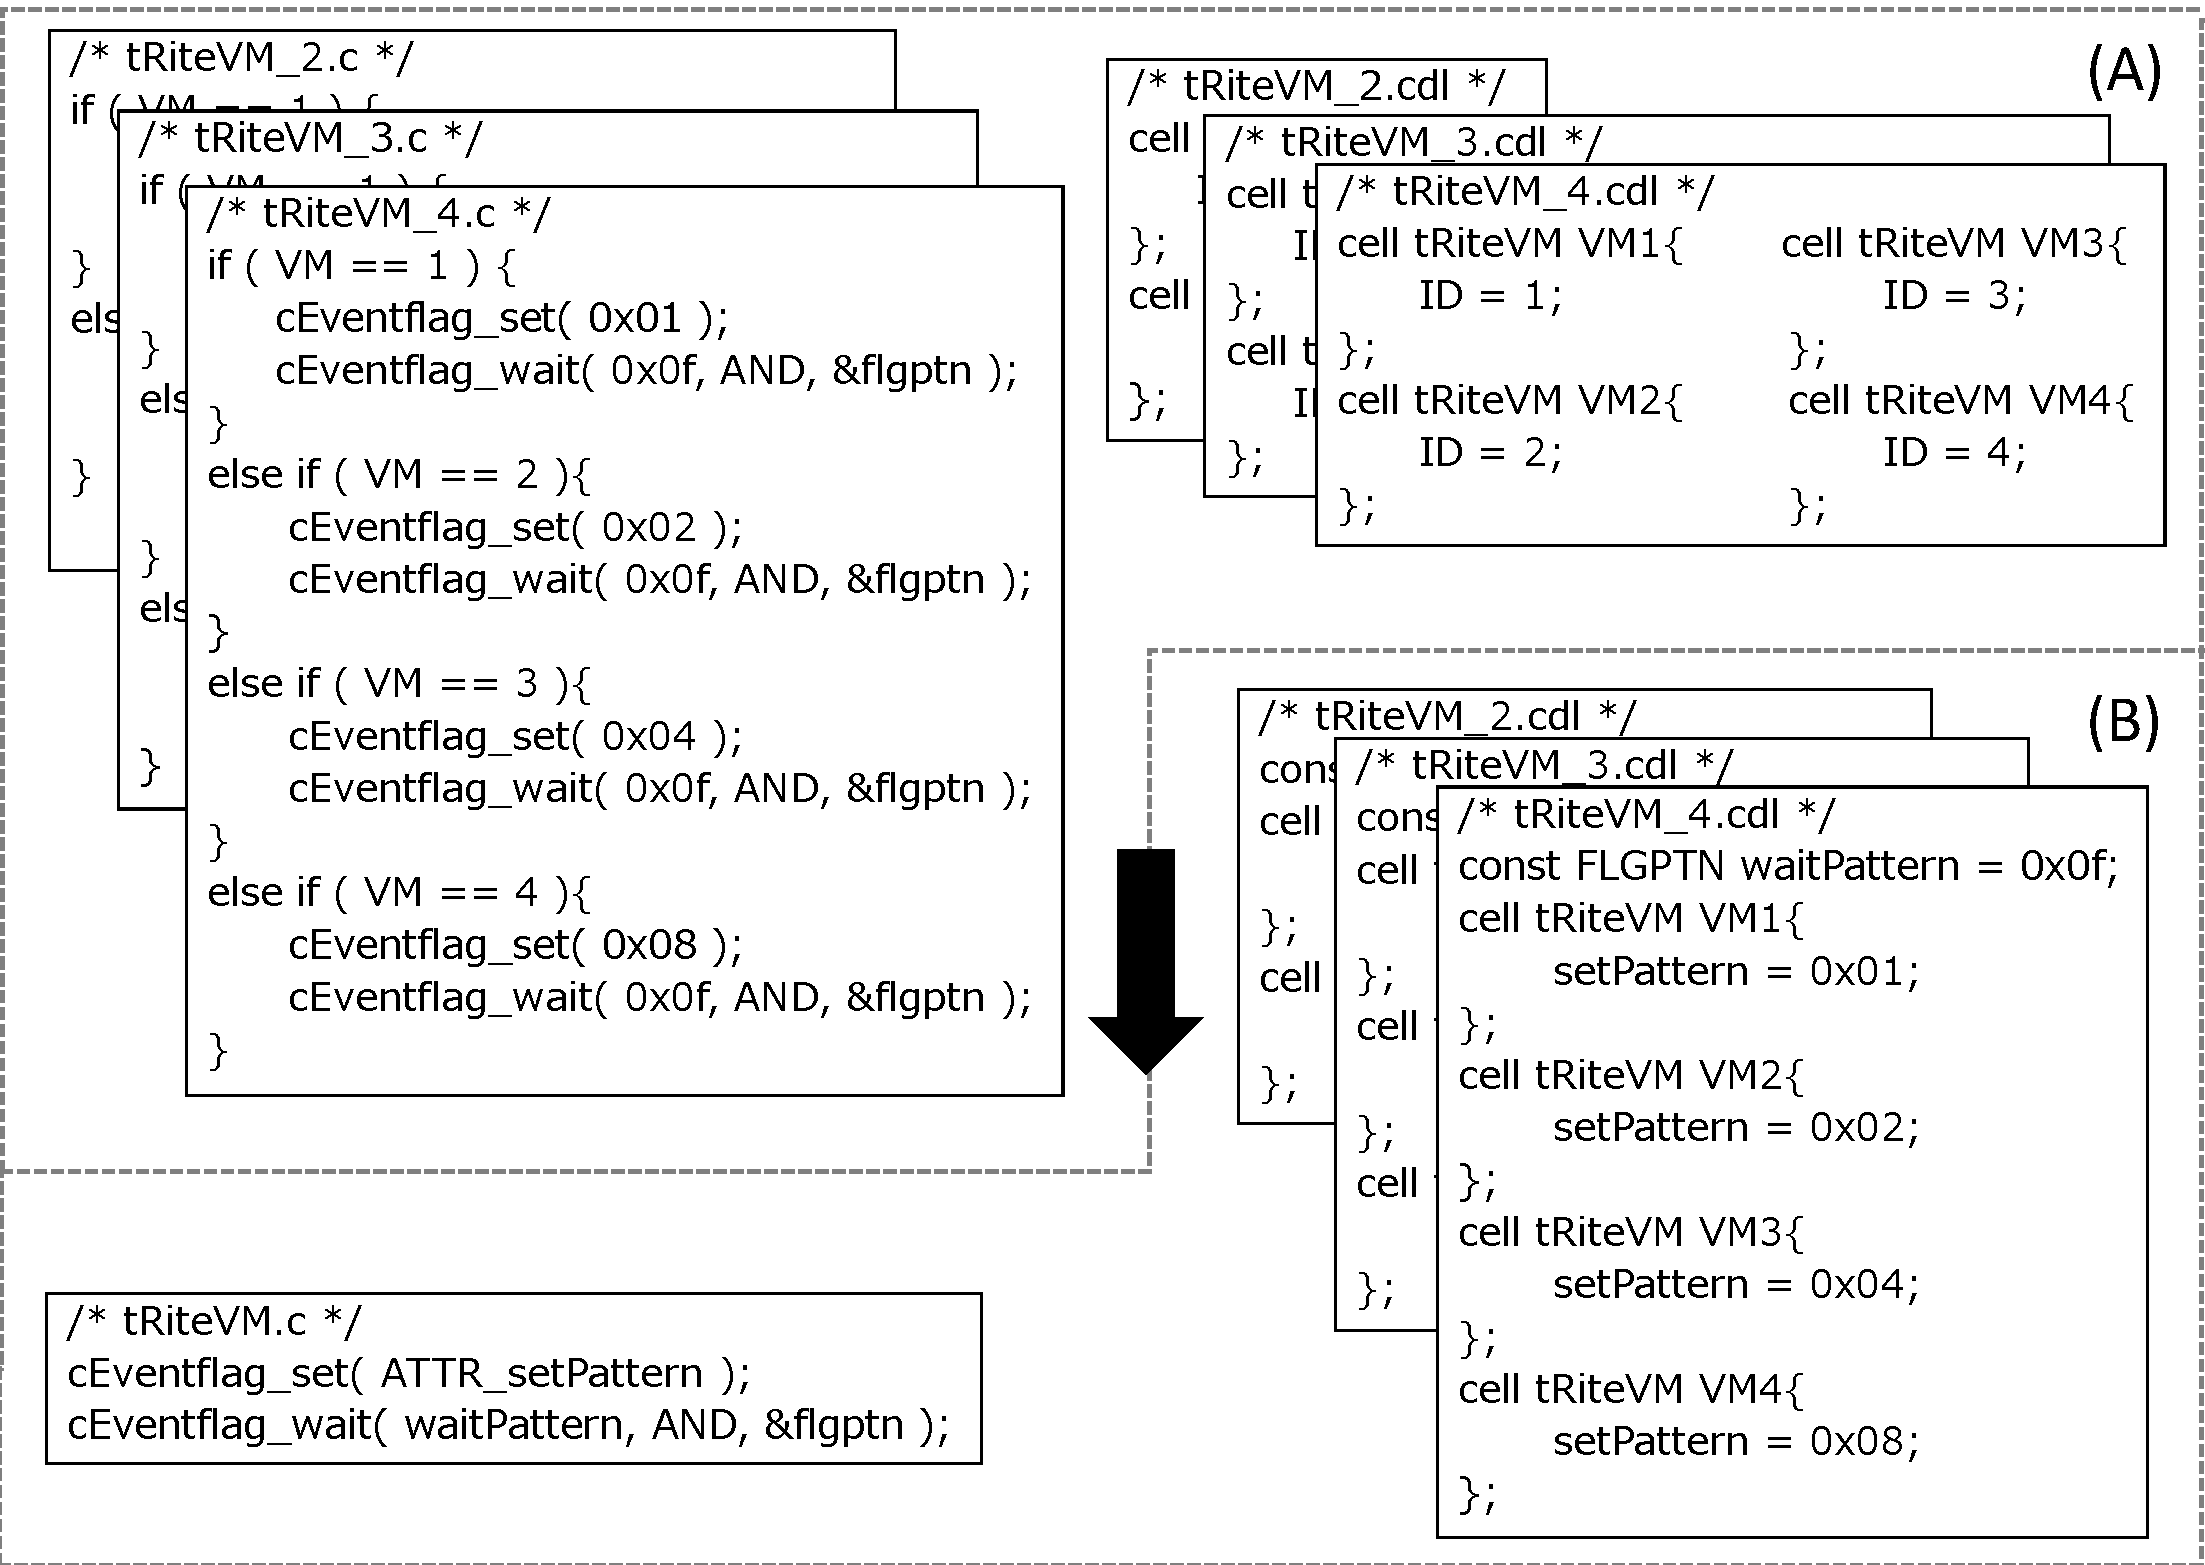
\includegraphics[width=8cm,clip]{../EMSOFT2016/figure/Eventflag.pdf}
    \caption{TECSを用いたイベントフラグの設計 {\scriptsize *差分のみ示す}}
\vspace{-2mm}
    \label{fig:Eventflag}
\end{figure}
 
\subsection{コンポーネントベース開発の利点}
この章では,コンポーネントベース開発の利点を使った設計について述べる.
提案フレームワークでは,RiteVMやRiteVMスケジューラ,イベントフラグはコンポーネントとして提供されているため,開発者はそれらのコンポーネントを容易に付け外し,再利用することができる.
例えば,RiteVMスケジューラの機能を外したい場合,図\ref{build_cyclic_handler}に示されるcdlファイルを{\it //import($<$tRiteVMScheduler.cdl$>$);}のようにコメントアウトすることで容易に実現できる.
開発者は,カーネルのコンフィグレーションファイルを修正する手間を省くことができる.

それに加えて,コンポーネントベース開発ではコード量を減らすことができる.
図\ref{fig:Eventflag}に示されるように,イベントフラグのセットパターンと待ちパターンを属性として定義する.
{\it cEventflag\_set(ATTR\_setPattern)}に見られるこの設計によって,if文なしでプログラムを記述でき,RiteVMの数に関わらず同じCファイルを使用できる.
さらに,TECSのオプションである{\it [optional]}によって,呼び口が結合した場合のみ処理を行うため,イベントフラグの結合を切った場合にでも同じCファイルを利用することができる.

\section{評価実験}
\vspace{-2mm}
\label{sec:Evaluation}
この章では,評価実験の結果と考察について述べる.
提案フレームワークの利点を分析するため,以下の評価を行った.
\begin{itemize}
%    \item プラットフォームの起動時間
    \item 転送されるmrubyバイトコードのサイズと処理時間およびコンパイル時間
    \item シングルタスク,コルーチン,マルチタスクの実行時間
    \item 周期時間によるオーバヘッド
%   \item mrubyアプリケーションの同期
    \item コンポーネントベース開発を利用したコード行数
\end{itemize}

% These evaluations are performed in order to indicate that an mruby bytecode loader improves the software development efficiency, and that the proposed multitask processing effectively executes compared with singletasking or co-routine, and also the overhead of the cyclic period.
本評価実験は,ターゲットデバイスとして,LEGO MINDSTORMS EV3 (300MHz ARM9-based Sitara AM1808 system-on-a-chip)を使用した.
コンパイラは,gcc 4.9.3 -O2 および mrubyのバージョンは,1.2.0である.

表\ref{tab:size_and_time}に,mrubyアプリケーションのバイトコードと,mrubyライブラリとアプリケーションのバイトコードのサイズ,ロードにかかる処理時間,コンパイル時間の比較を示す.
0バイトのバイトコードを処理した場合にかかるロード処理時間のオーバヘッドは,50.933 msecである.
同様に0バイトのバイトコードをコンパイルした場合にかかるコンパイルのオーバヘッドは,46.9 msecである.
mrubyアプリケーションのみのバイトコードの方が,ライブラリを含めた場合よりも,すべての点で優れている.
これはRiteVMひとつの評価であるため,RiteVMの数が増えるにつれ,この差は広がっていく.
さらに,この設計では,SDカードやROMを上書きしたり,OSを再起動する手間も省くことができる.
以上より,提案フレームワークは,既存フレームワークより作業効率を向上させることができる.

% The size, load process time, and compilation time for mruby application and mruby application including library is shown in Table \ref{tab:size_and_time}.
% The overhead of load processing is 50.933 msec, which it takes to load a zero bytes bytecode.
% Similarly, the overhead of compilation is 46.9 msec, which it takes to compile a zero bytes program.
% The mruby application bytecode is smaler and faster than that of including mruby libraries in all terms.
% The difference becomes larger as the number of RiteVMs increases because it takes the 50 msec overhead per one RiteVM. 
% %In the proposed framework, developers send only mruby application and prepare mruby library in advance.
% %Therefore, the design can send the bytecode faster.
% In addition, the design can save the time to connect a storage/ROM device to restart an OS.
% These advantages lead improvement of the software development efficiency.

\begin{table}[t]
    \centering
    \caption{転送されるmrubyバイトコードのサイズと処理時間およびコンパイル時間}
    {\tabcolsep=0.1cm
    \begin{tabular}{c||c|c|c}
                            & App\&Lib     & App        &   App\&Lib/App  \\ \hline
          Bytecode Size     & 14,044 bytes & 199 bytes  &   $\times$70.6          \\ %\hline
          Load Process Time & 305.081 msec & 7.774 msec &   $\times$39.2          \\
          Compile Time      & 8.7 msec     & 0.3 msec   &   $\times$29.0          \\
    \end{tabular}
    }
    \vspace{-3mm}
    \label{tab:size_and_time}
\end{table}

次に,図\ref{fig:comparison_s_c_m}に,シングルタスク,コルーチン,マルチタスクの実行時間を示す.
評価用のアプリケーションとして,100,000回ループするプログラムを適用し,マルチタスクおよびコルーチンは,2つのタスクでそれぞれ50,000回ループするプログラムを用いた.
実行時間の観点では,提案手法のマルチタスクは,シングルタスクよりも遅いが,コルーチンより有効である.
RiteVMスケジューラのオーバヘッドは,約5\%である.
タスクの切り替えそのものにかかる時間は,約3$\mu$secである.
RiteVMスケジューラは,周期的に割り込み,タスクの切り替えの処理を行うため,これがオーバヘッドとなっている.

% The comparison of the application execution time with singletasking, co-routine, and multitasking is shown in Figure \ref{fig:comparison_s_c_m}.
% The 100,000 times loop program is used as mruby application for evaluation of execution time.
% In detail, the singletask program loops 100,000 times, and the multitask and co-routine programs loop 50,000 times in each task.
% In Figure \ref{fig:comparison_s_c_m}, the cyclic time of the cyclic handler for multitasking is one msec.
% While multitask's execution time is slower than singletask's, co-routine takes more time than multitask to execute an mruby application.
% This result shows the proposed design is superior to co-routine in terms of execution time.
% The overhead of multitask is about 5 \% ($(multitask-singletask)/multitask$).
% Switching tasks' overhead is also evaluated, that is about three $\mu$sec on average.
% %The number of switching tasks is from 500 to 600 because singletasking process in Figure \ref{fig:comparison_s_c_m} takes about 540 msec.
% %Therefore, the overhead of multitasking is 0.5 \% or less, and multitasking can be used without the overhead.
% The scheuler interrupts and switches tasks, which causes this overhead.


\begin{figure}[t]
    \centering
    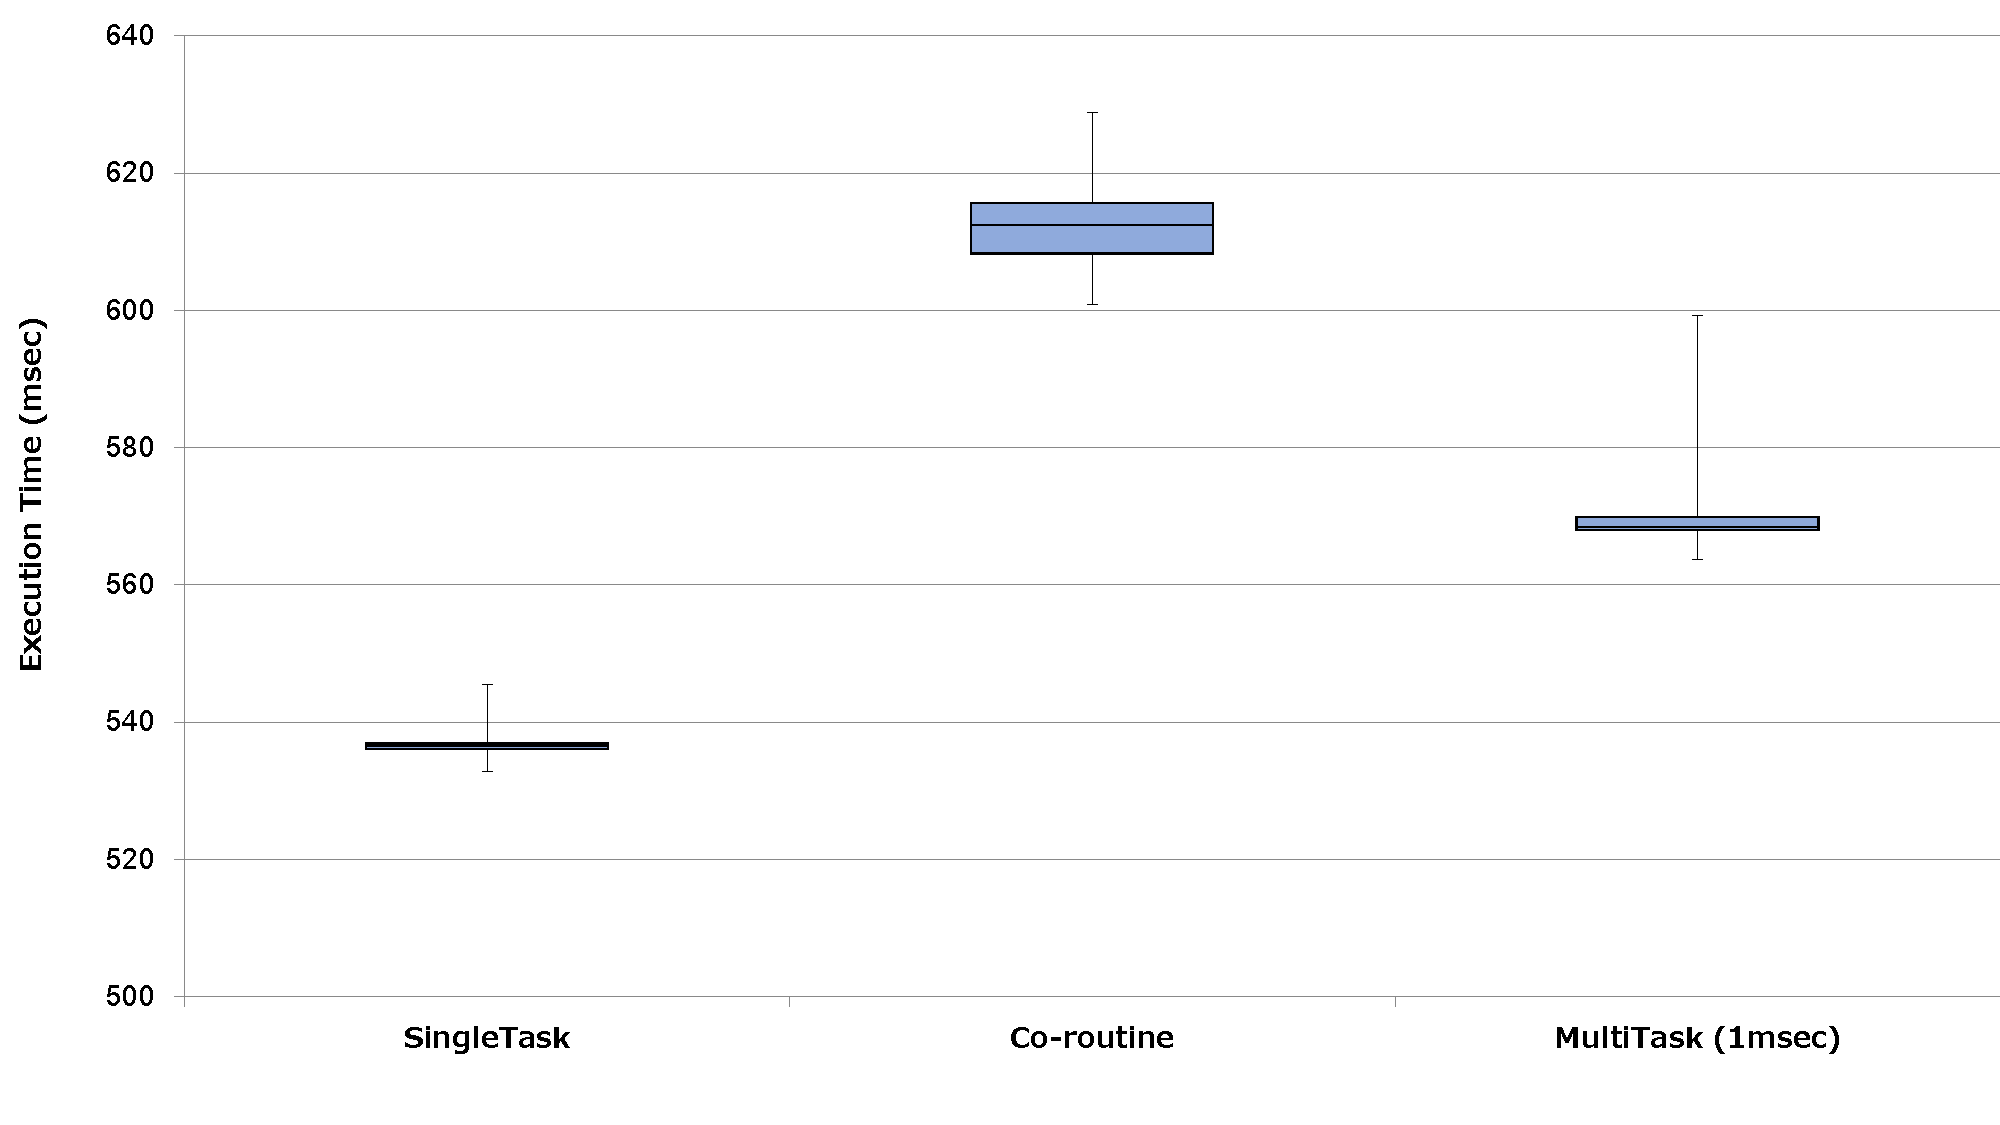
\includegraphics[width=8cm,clip]{../EMSOFT2016/figure/comparison_s_c_m.pdf}
    \caption{シングルタスク,コルーチン,マルチタスクの実行時間}
\vspace{-2mm}
    \label{fig:comparison_s_c_m}
\end{figure}

図\ref{fig:comparison_msec}は,RiteVMスケジューラの周期時間ごとの実行時間を示している.
この評価では,TOPPERS/HRP2の仕様により周期時間の下限を1msecとした.
また,周期時間が大きいとアプリケーションに影響を与える可能性があるため,上限を10msecとした.
周期時間が大きいほど,タスクの切り替え回数は減少するため,実行時間は小さくなることが分かる.
1msecと10msecでは,約3\%減少している.
1msecと8msecでは,約1\%減少している.
タスクを並行動作させるには,より小さい周期時間の方が好まれるが,オーバヘッドは大きくなる.
しかし,周期時間によるオーバヘッドは,誤差に埋もれるほど小さい.

% Figure \ref{fig:comparison_msec} shows the execution time of multitasking with the cyclic handler.
% A lower limit of the cyclic time is one msec due to the specification of TOPPERS/HRP2, the used RTOS.
% More than 10 msec do not be evaluated in this paper because it is thought the larger cyclic time influences applications.
% Each execution time of cyclic period is the same as the others.
% That is because the overhead of switching tasks (about 3 $\mu$sec) is small in comparison with the execution time.
% This results also shows the overhead becomes smaller as the cyclic time is larger, because the overhead depends on the number of switching tasks.
% The smaller cyclic time is better in multitasking due to concurrent and/or parallel processing.

\begin{figure}[t]
    \centering
    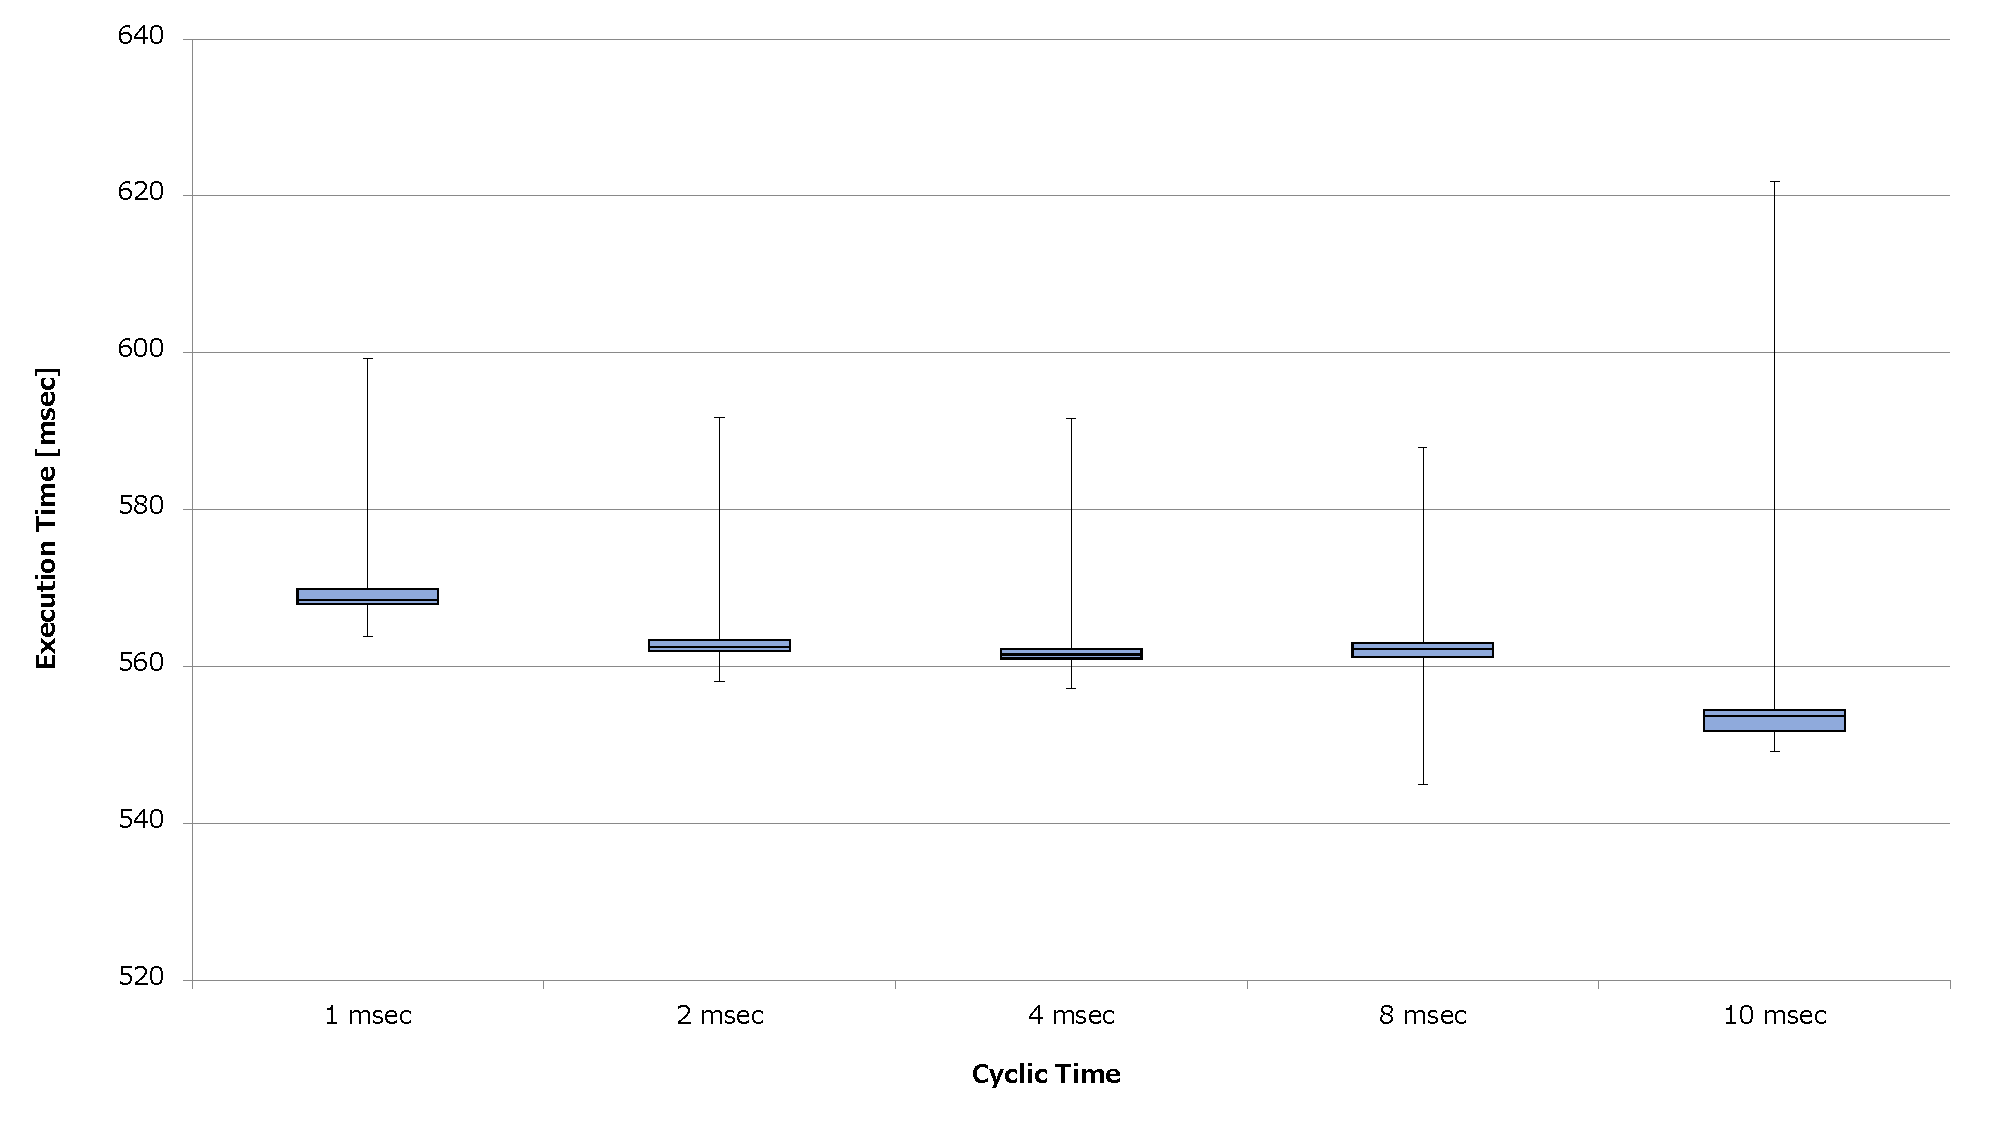
\includegraphics[width=8cm,clip]{../EMSOFT2016/figure/comparison_msec.pdf}
    \caption{周期時間によるオーバヘッド}
\vspace{-2mm}
    \label{fig:comparison_msec}
\end{figure}

表\ref{tab:codesize}に,2つの.cファイルと.cdlファイルのコード行数と変更行数の比較を示す.
(A)と(B)はそれぞれ,図\ref{fig:Eventflag}の上部と下部を指している.
(A)の.cファイルは,RiteVMの数に比例して増えているのに対して,(B)の.cファイルは同じである上に,RiteVMの数にかかわらず,修正することなく同一のファイルを使用できる.
さらに,.cdlファイルは両者違いはない.
コンポーネントベース開発を上手く活用することで,コードの行数を減らすことができ,高い生産性やメンテナンス性につながる.
その上,同じ.cファイルを利用できるため,開発者がファイルを修正する手間を省くことも可能になる.

% To indicate the superior of component-based development, the comparison of code lines between two .c files is shown in Table \ref{tab:codesize}.
% (A) and (B) mean the source files in the upper and lower of Figure \ref{fig:Eventflag}, respectively. 
% In terms of .c, (B)'s lines do not increase even if the number of RiteVMs increases, while (A)'s lines increase in proportion to the number.
% (B) is not modified, and can be utilized regardless of the number of RiteVMs.
% Moreover, lines of two .cdl files are equal.
% The skillfull component-based development brings this advantage such as the decrease of code lines, which leads high productivity and high maintainability.

\begin{table}[t]
    \centering
    \caption{コンポーネントベース開発を利用したコード行数} 
    \begin{tabular}{c||cc|c}
                & (A)       & (B)     & Diff  \\ \hline
        .c (Total)      & 8$\times$$\alpha$$+$134  & 130     & 8$\times$$\alpha+$4\\
        .c (Modified)   & 10$\times\alpha$$-$2 & 0   &  10$\times\alpha$$-$2 \\
        .cdl    & 18$\times$$\alpha$$+$25   & 18$\times$$\alpha$$+$25 & 0     \\
        %\multicolumn{3}{l}{  }\\
        \multicolumn{3}{l}{{\small $\alpha$} : {\scriptsize the number of RiteVM}}
    \end{tabular}
    \vspace{-3mm}
    \label{tab:codesize}
\end{table}

\section{関連研究}
\vspace{-2mm}
\label{sec:Related Work}

% \begin{table*}[t]
%     \centering
%     \caption{関連研究}
%     {\tabcolsep=0.1cm
%     \begin{tabular}{c||c|ccccccc}
%         & Bluetooth Loader & \shortstack{Call\\C Function} & \shortstack{Legacy Code of\\Embedded System} & \shortstack{VM\\Managenment} & \shortstack{VM\\Scheduler} & \shortstack{Synchronization of\\Application} & Co-routine \\ \hline
%         python-on-a-chip\cite{url:python-on-a-chip} &            &            &            &            &             &            & \checkmark \\
%         Owl system\cite{par:owl}                    &            & \checkmark & Partially  &            &             &            & \checkmark \\
%         eLua\cite{url:eLua}                         &            & \checkmark & Partially  &            &             &            & \checkmark \\
%         mruby\cite{par:mruby}                       &            & \checkmark &            &            &             &            & \checkmark \\
%         mruby on TECS\cite{par:mrubyonTECS}         &            & \checkmark & \checkmark & \checkmark &             &            & \checkmark \\
%         Proposed framework                           & \checkmark & \checkmark & \checkmark & \checkmark & \checkmark  & \checkmark & \checkmark \\
%     \end{tabular}
% }
%     \label{tab:comparison}
% \end{table*}
現在,オープンソースのスクリプト言語のランタイムシステムとして,次のものが開発されている.
python-on-a-chip\cite{url:python-on-a-chip}, the Owl system\cite{par:owl}, eLua\cite{url:eLua}, mruby\cite{par:mruby},\cite{url:mruby}, mruby on TECS\cite{par:mrubyonTECS}.

python-on-a-chip(p14p)は,PyMyteと呼ばれるPythonVMを使用する,Pythonランタイムシステムである.
PyMyteは,マイクロコントローラー上で低リソースでPythonプログラムを実行する.
p14pは,スタックレスなグリーンスレッドを複数動作させることができる.

Owl systemは,組込みシステム向けのPythonランタイムシステムであり,ARM Cortex-M3 マイクロコントローラー上で動く.
Owlツールチェーンは,Pythonコードから,マイコン上で直接起動するメモリイメージを生成する.
Owl systemは,p14pのインタプリタを使用している.

eLuaは,Luaを組込みシステム向けの完全な実装である.
%Luaは,最も人気のある組込み向けスクリプト言語のひとつである\cite{url:Lua}, \cite{par:Lua}.
Luaは,協調的マルチタスク処理が可能なコルーチンをサポートしているが,コルーチンは,ノンプリエンプティブであるため,マルチタスク処理のようなプログラムを行うのは難しい.

%mruby(軽量Ruby)は,組込みシステムに適したスクリプト言語である.
%mrubyプログラムは,RiteVM上で実行される.
mrubyは,コルーチンをサポートしているが,RTOSのマルチタスクには対応していない.

%mruby on TECSは,mrubyを使ったコンポーネントベース開発が可能なフレームワークである.
%mruby on TECSは,mrubyより実行速度が100倍速い.
mruby on TECSは,マルチタスクをサポートしているが,マルチタスク処理を行うには,開発者がRTOSの機能を呼び出す必要がある.

%表\ref{tab:comparison}に,提案フレームワークと既存研究の比較を示す.
提案フレームワークでは,ローダに加えて,VMスケジューラとアプリケーションの同期機構を提供する.

\section{おわりに}
\vspace{-2mm}
\label{sec:Conclusion}
本研究では,mruby on TECSの拡張として,Bluetoothを用いたmrubyバイトコードローダとRiteVMスケジューラを提案した.
mrubyバイトコードローダによって,開発者はSDカードやROMを上書きしたり,OSを再起動する手間が省けるため,mruby on TECSでのソフトウェア開発の作業効率を向上させる.
ローダは,Bluetoothだけでなく,有線のシリアル通信にも対応しているため,様々な組込みシステムに適用できる.
RiteVMスケジューラは複数のmrubyアプリケーションを効率良く並行実行する.
実験評価では,ローダによる作業効率の向上やオーバヘッドの少ないマルチタスク設計の有用性,コンポーネントベース開発の利点を示した.

さらに,提案フレームワークで提供される機能はコンポーネントであるため,機能の取り外しや再利用が容易になる.
RiteVMスケジューラも容易に付け外しできるため,開発者は,フェアスケジューリングか固定優先度スケジューリングかを選択することもできる.
コンポーネントベース開発は,生産性を向上させ,システムの複雑さを減らすことができる.

ソフトウェア開発をさらに効率よく行うために,プラグインを使用したRiteVMやmruby-TECSブリッジの.cdlファイルの自動生成や,コマンドライン上でのバイトコードの転送などを提供することが,今後の課題である.

%%%%%%%%%%%% Reference %%%%%%%%%%%%%%%%%%%%%%%%%%%%%%%%%%%%%%%%%%%%%%
\vspace{-2mm}
\bibliographystyle{ipsj_v2/UTF8/ipsjunsrt-e}
\bibliography{ETNET}

% \begin{biography}
% \profile{m,E}{情報 太郎}{1970年生.1992年情報処理大学理学部情報科学科卒業.
% 1994年同大学大学院修士課程修了.同年情報処理学会入社.オンライン出版の研究
% に従事.電子情報通信学会,IEEE,ACM 各会員.}
% %
% \profile{n}{処理 花子}{1960年生.1982年情報処理大学理学部情報科学科卒業.
% 1984年同大学大学院修士課程修了.1987年同博士課程修了.理学博士.1987年情報処
% 理大学助手.1992年架空大学助教授.1997年同大教授.オンライン出版の研究
% に従事.2010年情報処理記念賞受賞.電子情報通信学会,IEEE,IEEE-CS,ACM
% 各会員.}
% %
% \profile{h,L}{学会 次郎}{1950年生.1974年架空大学大学院修士課程修了.
% 1987年同博士課程修了.工学博士.1977年架空大学助手.1992年情報処理大学助
% 教授.1987年同大教授.2000年から情報処理学会顧問.オンライン出版の研究
% に従事.2010年情報処理記念賞受賞.情報処理学会理事.電子情報通信学会,
% IEEE,IEEE-CS,ACM 各会員.}
% \end{biography}

\end{document}
